\chapter{On genus one}

\section{Reduced invariants and the Li-Zinger's formula}
Contrary to the genus zero case, $\M{1}{n}{\PP^N}{d}$ is not a smooth stack; in fact it is not even equidimensional. A classical example is given by $\M{1}{0}{\PP^2}{3}$:
\begin{itemize}
 \item smooth planar cubics are elliptic curves by the degree-genus formula; viewing them as $E\hookrightarrow \PP^2$ gives a component of dimension $9$ of $\M{1}{0}{\PP^2}{3}$, often referred to as the \emph{main} component;
 \item a contracted elliptic curve attached to a rational tail that normalises a nodal cubic determines the generic point of a different component of dimension $10$, which I am going to denote by $D^1(\PP^2,3)$;
 \item finally a contracted genus one curve with two rational tails parametrising the union of a line and a quadric in $\PP^2$ describes the generic element of yet another $9$-dimensional component, that I shall denote by $D^2(\PP^2,3)$.
\end{itemize}
Furthermore, the boundary of the main component admits a neat description: $\M{1}{0}{\PP^2}{3}^{\mathrm{main}}\cap D^1(\PP^2,3)$ consists of those maps where the rational tail normalises a cusp, and the elliptic curve is contracted exactly to the singular point (this has dimension $8$, thus being a divisor in \emph{main}); while $\M{1}{0}{\PP^2}{3}^{\mathrm{main}}\cap D^2(\PP^2,3)$ has the line tangent to the conic.

The description above generalises indeed to all moduli spaces of maps to $\PP^N$ in genus one:
besides the \emph{main component}, which is the closure of the locus of maps from a smooth elliptic curve, for every positive integer $k$ and partition $\lambda\vdash d$ into $k$ positive parts, there is an irreducible \emph{boundary component} $D^{\lambda}(\PP^N,d)$ defined to be the closure of the locus where:
\begin{enumerate}[label=(\roman*)]
\item the source curve is obtained by gluing a smooth $k$-pointed elliptic curve $E$ with as many rational tails $R_i\cong\PP^1,\ i=1,\ldots,k$,
\item the map contracts the elliptic curve $E$ to a point, 
\item the map has degree $\lambda_i$ on the rational tail $R_i$.
\end{enumerate}
$D^{\lambda}(\PP^N,d)$ is irreducible, being the image of the gluing morphism from
\[\left(\oM_{1,k}\times\prod_{i=1}^k\M{0}{1}{\PP^N}{\lambda_i}\right)\times_{(\PP^N)^k}\PP^N.\]
I will denote by $D^k(\PP^N,d)$ the union of all $D^{\lambda}(\PP^N,d)$ where $\lambda$ has $k$ parts. An analogous description holds in the case of a positive number of markings, except that the combinatorial data should also include a partition $\mu\vdash n$ into $k+1$ parts (the $0$-th of which telling how many points lie on $E$).

 %We then have:
\begin{prop}\label{prop:components} The minimal connected arithmetic genus one subcurve is named the \emph{core} (it could consist of a circle of $\PP^1$).
\begin{enumerate}
 \item The ones above are all the irreducible components of $\oM_1(\PP^N,d)$: 
\[\oM_1(\PP^N,d)=\oM_1(\PP^N,d)^{\rm{main}}\cup\bigcup_{\lambda}D_{\lambda}(\PP^N,d).\]
\item A map $[f]$ lies in \emph{the boundary of the main component}  if and only if:
\begin{itemize}[leftmargin=0cm]
\item $f$ is non-constant on at least one irreducible component of the core,
\item or, if $f$ contracts the core, writing $C=Z\ {}_{\mathbf p}\!\sqcup_{\mathbf q}\bigsqcup_{i=1}^k R_i$ with $Z$ the \emph{maximal} contracted subcurve of genus one, then $\{\operatorname{d}\!f(T_{q_i}R_i)\}_{i=1}^k$ is a \emph{linearly dependent} set in $T_{f(Z)}\PP^r$.
\end{itemize}
In this case we say that $[f]$ is smoothable.
\end{enumerate}
\end{prop}
 
This is essentially due to R. Vakil and A. Zinger, see \cite[Lemma~5.9]{Vre} \cite[\S 1.2]{VZ}. Later I shall discuss a proof of the second fact based on local equations for the moduli space.

Let me carry the comparison to the genus zero situation one step further: assume we are interested in the Gromov-Witten theory of a complete intersection in $\PP^N$, say a hypersurface $X$ of degree $l$, cut out by a section $s\in H^0(\PP^N,\OO_{\PP^N}(l))$. Letting $(\pi,f)\colon \mathcal C_{0,n}(\PP^N,d) \to \M{0}{n}{\PP^N}{d}\times \PP^N$ denote the universal curve and stable map, recall that there is an induced section $\tilde{s}$ of the sheaf $E=\pi_*f^*\OO_{\PP^N}(l)$ on $\M{0}{n}{\PP^N}{d}$, which vanishes along $\M{0}{n}{X}{d}$. In fact more is true: $E$ is a vector bundle of rank $dl+1$ (by cohomology and base-change, and a Riemann-Roch computation) and, after shifting, it provides us with a perfect obstruction theory for the inclusion $\iota\colon \M{0}{n}{X}{d}\hookrightarrow\M{0}{n}{\PP^N}{d}$, so that the following result holds.

\begin{prop}\cite{CKL,KKP}
 With notation as above,
 \[\iota_*\virt{\M{0}{n}{X}{d}}=c_{dl+1}(E)\cap [\M{0}{n}{\PP^N}{d}].\]
\end{prop}
In particular, this result makes the restricted Gromov-Witten invariants of $X$ into \emph{twisted} Gromov-Witten invariants of projective space, thus computable e.g. by localisation \cite{Kon}.

Again the situation in genus one is much more intricate: $\pi_*f^*\OO_{\PP^N}(l)$ generically has rank $dl$ on the main component, but the rank jumps to $dl+1$ on the boundary, where the elliptic curve is contracted - as can be seen by constancy of the Euler characteristic and the fact that $\operatorname{R}^1\pi_*f^*\OO_{\PP^N}(l)$, that always satisfies cohomology and base-change, is supported on such boundary loci. In other words, the natural obstruction theory for $\M{1}{n}{X}{d}\hookrightarrow\M{1}{n}{\PP^N}{d}$ is not perfect.

A possible approach to this problem is the one taken by J. Li, R. Vakil and A.Zinger in a series of papers \cite{zsharp,zstructure,redgone,LZ,lz2,zingerstvsred,VZpreview,VZ}: roughly, they produce a \emph{desingularisation} $\VZ{n}{\PP^N}{d}$ of the main component, on which the cone $\pi_*f^*\OO_{\PP^N}(l)$ is seen to contain a vector bundle $E$ of rank $dl$, and for a hypersurface $X_l\subseteq \PP^N$ as before (more generally for a projective complete intersection) they define \emph{reduced invariants} by integrating against
\[\redu{\iota_* \VZ{n}{X}{d}}:= c_{dl}(E)\cap [\VZ{n}{\PP^N}{d}].\]
Reduced invariants may be computed by torus localisation as well \cite{Zinger-CYhyp,APopa}. Let me describe Vakil and Zinger's construction more precisely: it is an iterated blow-up that makes all the boundary components intersect \emph{main} in a divisor (within the latter). Let $\Mwt$ denote the stack of prestable curves with a weight assignment, namely to every irreducible component in the fiber we associate a non-negative integer in a way compatible with specialisation morphisms: $\Mwt$ is \'etale but non-separated over $\MM_1$, and it was first considered by \cite{Costello} By a slight abuse of notation I will also denote by $\Mwt$ the open, bounded locus where the curve is weighted-stable, i.e. every rational component of weight zero has at least three special points. $\M{1}{n}{\PP^N}{d}$ admits a map to $\Mwt$ by retaining only the degree of the map. Let $\Theta_k\subseteq \Mwt$ denote the closure of the locus where the elliptic curve has weight zero, and $k$ rational tails of positive weight attached to it. Define $\MM^{(0)}=\Mwt$ and $\MM^{(k)}$ iteratively as the blow-up of the strict transform of $\Theta_k$ in $\MM^{(k-1)}$. Notice that the blow-up loci are always smooth, hence so is $\MM^{(k)}$ for every $k$; also, by weighted-stability, for every fixed total degree $d$ the procedure stops after finitely many steps: denote by $\widetilde{\MM}$ the end result. Form the cartesian diagram
\bcd
\tVZ{n}{\PP^N}{d}\ar[d]\ar[r]\ar[dr,phantom,"\Box"] & \M{1}{n}{\PP^N}{d}\ar[d] \\
\widetilde{\MM}\ar[r] & \Mwt
\ecd
Now the pullback of any boundary component of $\M{1}{n}{\PP^N}{d}$ has the same dimension in $\tVZ{n}{\PP^N}{d}$ and intersects its main component (which is denoted by $\VZ{n}{\PP^N}{d}$ and is smooth \cite[Theorem 1.1(1)]{VZ}\cite[Theorem 2.9]{HL}) in a Cartier divisor. Denoting $\mathcal L=\tilde f^*\OO_{\PP^N}(1)$ on the universal curve, notice that $\R\pi_*\mathcal L$ may be resolved locally by picking a smooth section $\mathcal A$ of the universal curve passing through the core and writing:
\[0\to \tilde\pi_*\mathcal L\to \tilde\pi_*(\mathcal L\otimes \OO_{\mathcal C}(\mathcal A))\xrightarrow{\mathrm{res}_{\mathcal A}} \tilde\pi_*(\mathcal L(\mathcal A)_{|\mathcal A})\to \operatorname{R}^1\tilde\pi_*\mathcal L\to 0\]
By restricting to $\VZ{n}{\PP^N}{d}$ we see then that the image of the middle arrow is $\tilde\pi_*(\mathcal L(\mathcal A)_{|\mathcal A})(-\Xi)$ where $\Xi$ denotes the boundary of the main component of the Vakil-Zinger's desingularisation, hence $\tilde\pi_*\mathcal L$ is a vector bundle (being the kernel of a vector bundle morphism). A similar argument works for all the tensor powers of $\mathcal L$, and in particular we let $E:=\tilde\pi_*\mathcal L^{\otimes l}$. The previous discussion can be made accurate by studying the arrow $\mathrm{res}_{\mathcal A}$ in local coordinates \cite[Proposition 4.13]{HL}.

It is clear from the construction above that reduced invariants ought to have a better enumerative meaning than ordinary Gromov-Witten invariants, in the sense that they discard most boundary contributions from nodal curves. In the realm of symplectic geometry, it has been proven by Li and Zinger \cite{LZ} that for every \emph{primary} insertion $(\delta_1,\ldots,\delta_n)\in H^*(X)^{\otimes n}$ and curve class $\beta\in H^+_2(X)$
\[
 \langle \delta_1,\ldots,\delta_n \rangle^X_{1,n,\beta}-\langle \delta_1,\ldots,\delta_n \rangle^{X,\mathrm{red}}_{1,n,\beta}=\begin{cases}
 0 & \text{if } \dim(X)=2, \\
 \frac{2-K_X\cdot\beta}{24}\langle \delta_1,\ldots,\delta_n \rangle^X_{0,n,\beta} & \text{if } \dim(X)=3.\end{cases}
\]
Li-Zinger's equation tells us that in the case of a threefold, which is the most natural one where to look for such a comparison result because the virtual dimension (hence the meaningful insertions) does not depend on the genus, the difference between ordinary and reduced genus one invariants is given by the corresponding genus zero invariant multiplied by a correction factor. The relation has been proved in algebraic geometry for the quintic threefold \cite{CL}, and it is an extension of this project that I am going to discuss in the next few sections. Together with Cristina Manolache and Tom Coates I am also working towards a different proof of the formula: the key issue is to prove that the components of the intrinsic normal cone supported on the boundary components compare well (as in \cite{Manolache-push}) to their genus zero relatives, excluding those that do not contribute at all. I shall not attempt a detailed discussion here; I will rather work out the case of projective spaces of low dimension, which can be dealt with entirely by hand. Let me recall the following
\begin{lemma}\cite[Proposition 1.8]{Ful}
Let $U\overset{j}{\hookrightarrow} X \overset{i}{\hookleftarrow} Z$ be complementary open and closed subvarieties. Then the following sequence is exact:
\[A_k(Z)\overset{i_*}{\to} A_k(X)\overset{j^*}{\to} A_k(U)\to 0\]
\end{lemma}
This means that, whenever we are studying a virtual cycle of dimension $d$, we are allowed to disregard any closed substack of dimension less than $d$. Furthermore cones and Gysin pullbacks behave well under restriction to open subsets \cite[Proposition 4.2(b) and Theorem 6.2(b)]{Ful}. Also $\tVZ{n}{\PP^N}{d}\to \M{1}{n}{\PP^N}{d}$ is virtually birational, and all the insertions come from downstairs.  

Let me start by loooking at $\M{1}{n}{\PP^1}{d}$. Except for $d=1$, where the main component is empty, there are $n+2$ components: the main one and a boundary component for every partition of $n$ into two parts, which is the image of gluing \[\oM_{1,k+1}\times\M{0}{n-k+1}{\PP^1}{d}.\]
All components have the same dimension, which is also equal to the virtual dimension; this in particular means that we can discard all the intersections, so that every component of what remains is smooth. From the exact triangle
\[ E^\bullet_{\oM(\PP^1)/\MM}\to E^\bullet_{\oM(\PP^1)}\to \rho^*T^\bullet_{\MM}\overset{[1]}{\to}\]
observe that the relative obstruction space $\mathbb E^\vee\boxtimes \ev_q^*T_{\PP^1}$ - where $\mathbb E$ is the Hodge bundle and $q$ is the gluing node - cancels out with the normal bundle of the boundary divisor in the moduli space of curves, which is $\mathbb L_{q,E}^\vee\boxtimes \mathbb L_{q,R}^\vee$ - where $\mathbb L_{p,C}$ denotes the cotangent line of the curve $C$ at the smooth point $p$. Notice that the difference between $\lambda_1$ and $\psi_1$ (when there are markings on the elliptic tail) is supported precisely on the intersection with the other boundary components, while $\operatorname{d}\!f_q$ gives an isomoprhism $\mathbb L_{q,R}^\vee\xrightarrow{\sim}\ev_q^*T_{\PP^1}$, except when the gluing node is a ramification point for the map, which only happens at the intersection with \emph{main} by Proposition \ref{prop:components}. This shows that the virtual class is the sum of the fundamental classes of all the components. Clearly no boundary component will contribute to the primary invariants.

The case of $\PP^2$ is slightly more complicated: the boundary component $D^1$ has excess dimension $1$, and two irreducible components $D^{\lambda=(d),\mu=(A_0,A_1)}$ and $D^{\lambda,\mu'}$ intersect if and only if $A_0\subseteq A_0'$ and $A_1'\subseteq A_1$, or viceversa; in this case the dimension of the intersection is equal to the virtual dimension. Remark that $\operatorname{d}\!f_q\equiv 0$ along the intersection. Finally $D^2$ has dimension equal to the virtual one as well. Notice that $D^1$ is the pull back of the boundary divisor $\mathfrak{D}^1$ in $\MM_{1,n}^{\mathrm{wt}}$, and the projection $D^1\to \mathfrak{D}^1$ is smooth, so in particular the intrinsic normal cone of $D^1\setminus \M{1}{n}{\PP^2}{d}^{\mathrm{main}}$ is a vector bundle stack; we may therefore work componentwise on $D^1\setminus \M{1}{n}{\PP^2}{d}^{\mathrm{main}}$. Comparing the normal bundle of $\mathfrak{D}^1$ in $\MM_{1,n}^{\mathrm{wt}}$ with the obstruction bundle of $D^1$, it follows from an easy Chern class computation that \[c_1\left(\frac{\mathbb E^\vee\boxtimes \ev_q^*T_{\PP^2}}{\mathbb L_{q,E}^\vee\boxtimes \mathbb L_{q,R}^\vee}\right)=3\cdot1\boxtimes\ev_q^*H+2\cdot\lambda_1\boxtimes1-\psi\boxtimes1-1\boxtimes\psi\]
From arguments similar to the above ones we see that $D^2$ contributes with its fundamental class. We may wrap it all up in the following formula:
\begin{multline*}
 \langle \tau_{h_1}(H^{k_1}),\ldots,\tau_{h_n}(H^{k_n})\rangle^{\PP^2}_{1,n,d}= \langle \tau_{h_1}(H^{k_1}),\ldots,\tau_{h_n}(H^{k_n})\rangle^{\PP^2,\mathrm{red}}_{1,n,d}+\\
 \hspace{-2cm}\sum_{A_0\coprod A_1=[n]}\biggr(\langle \psi^{h^0_1},\ldots,\psi^{h^0_{n_0}},1\rangle^{\{*\}}_{1,A_0\cup \{q_E\}}\langle 3H^{\sum _{i\in A_0}k_i+1}-\tau_1(H^{\sum_{i\in A_0}k_i}),\tau_{h^1_1}(H^{k^1_1}),\ldots,\tau_{h^1_{n_1}}(H^{k^1_{n_1}})\rangle^{\PP^2}_{0,\{q_R\}\cup A_1,d}+\\
  \langle \psi^{h^0_1},\ldots,\psi^{h^0_{n_0}},2\lambda_1-\psi\rangle^{\{*\}}_{1,A_0\cup \{q_E\}}\langle H^{\sum _{i\in A_0}k_i},\tau_{h^1_1}(H^{k^1_1}),\ldots,\tau_{h^1_{n_1}}(H^{k^1_{n_1}})\rangle^{\PP^2}_{0,\{q_R\}\cup A_1,d}\biggr)+\\
 \hspace{-4.3cm}\sum_{\substack{A_0\coprod A_1\coprod A_2=[n]\\ d_1+d_2=d:\ d_1,d_2>0}}\sum_{j=0}^2\langle \psi^{h^0_1},\ldots,\psi^{h^0_{n_0}},1,1\rangle^{\{*\}}_{1,n_0+2}\langle H^{j+\sum _{i\in A_0}k_i},\tau_{h^1_1}(H^{k^1_1}),\ldots,\tau_{h^1_{n_1}}(H^{k^1_{n_1}})\rangle^{\PP^2}_{0,1+n_1,d_1}\langle H^{2-j},\tau_{h^2_1}(H^{k^2_1}),\ldots,\tau_{h^2_{n_2}}(H^{k^2_{n_2}})\rangle^{\PP^2}_{0,1+n_2,d_2}
\end{multline*}
Notice in particular that ordinary and reduced invariants coincide for primary insertions (using the string equation).

The case of $\PP^3$ is even more complicated: $D^1$ has excess dimension two, and $D^1$ has excess dimension $1$. They intersect in the locus of ``Mickey Mouse with an earring is eating a doughnut with a fly'' (the configuration of points is admittedly arbitrary).
\begin{figure}[h]
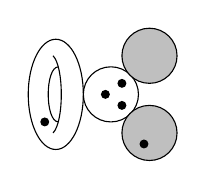
\begin{tikzpicture}[scale=.7]
\draw (0,0) circle (.5cm);
\draw[radius=2pt, fill=black] (.2,.2) circle;
\draw[radius=2pt, fill=black] (.2,-.2) circle;
\draw[radius=2pt, fill=black] (-.1,0) circle;

\draw[radius=2pt, fill=black] (-1.2,-.5) circle;
\draw[fill=gray!50] (.7,.7) circle (.5cm);
\draw[fill=gray!50] (.7,-.7) circle (.5cm);
\draw (-1,0) ellipse (.5cm and 1cm);
\draw (-1.05,.7) .. controls (-.85,.5) and (-.85,-.5) .. (-1.05,-.7);
\draw (-.95,.5) .. controls (-1.2,.5) and (-1.2,-.5) .. (-.95,-.5);
\draw[radius=2pt, fill=black] (.6,-.9) circle;
\end{tikzpicture}
\end{figure}
The local model for the space near such a boundary point is $V(xy,xz)\subseteq\Aaff^3_{x,y,z}$, where $D^1=\{x=0\}$ and $D^2={y=z=0}$. The normal cone \[\Spec\left(\kk[x,y,z][A,B]/(xy,xz,zA-yB)\right)\] has two components defined by $(y,z)$ (this is a rank-two vector bundle on $D^2$, coinciding with its normal bundle) and $(x,zA-yB)$: the latter is \emph{not} a line bundle on $D^1$, as it has rank two over the origin, so in particular it is not its normal bundle; on the other hand the cycle of this cone has dimension three, and its restriction to the origin has dimension two, so we may effectively delete it, and behave \emph{as if} it were just the normal bundle of $D^1$. We may therefore argue similarly as before, and we find that the relevant bundles are \[\frac{\mathbb E^\vee\boxtimes \ev_q^*T_{\PP^3}}{\mathbb L^\vee_{q,E}\boxtimes \mathbb L^\vee_{q,R}}\]
on $D^1$, of which we take $c_2$, while on $D^2$ we compute $c_1$ of \[\frac{\mathbb E^\vee\boxtimes \ev_q^*T_{\PP^3}}{\mathbb L^\vee_{q_1,E}\boxtimes \mathbb L^\vee_{q,R_1}\oplus\mathbb L^\vee_{q_2,E}\boxtimes \mathbb L^\vee_{q,R_2}}.\]
$D^3$ has dimension equal to the virtual dimension. A Chern class calculation implies (with schematic notation suggested by N. Nabijou):
\begin{multline*}
 \virt{\M{1}{n}{\PP^3}{d}}=[\reduced]+ 4[\Dunouno]+4[\Dunodue]+\\
 -3[\Dunotre]-3[\Dunoquat]+[\Dunocin]+2[\Dunosei]+\\
 [\Dunoset]+3[\Dunoott]-8[\Dunonov]+6[\Dunodiec]+\\
 4[\Ddueuno]-3[\Dduedue]+[\Dduetre]+[\Dduequat]+\\
 [\Dduecin]+[\Dduesei]+[\Dtre]
\end{multline*}
If we restrict our attention to primary invariants, the only survivors are:
\begin{multline*}
 [\reduced]+ 4[\Dunouno]-3[\Dunotre]-3[\Dunoquat]+\\
 [\Dunocin]+2[\Dunosei]+3[\Dunoott]-8[\Dunonov]
\end{multline*}
They contribute tidily as follows:
\begin{enumerate}
 \item gives the reduced invariants,
 \item $4\langle\psi\rangle_{1,1}\langle H,-\rangle^{\PP^3}_{0,n+1,d}=\frac{4d}{24} GW_0$ by divisor,
 \item $-3\langle\lambda_1\psi,1\rangle_{1,2}\langle -\rangle^{\PP^3}_{0,n,d}=\frac{-3n}{24} GW_0$ since there are $n$ choices for the marking on the genus one curve,
 \item $-3\langle\lambda_1\rangle_{1,1}\langle \psi,-\rangle^{\PP^3}_{0,n+1,d}=\frac{-3(n-2)}{24} GW_0$ by dilaton,
 \item $\langle\psi^2,1\rangle_{1,2}\langle -\rangle^{\PP^3}_{0,n,d}=\frac{n}{24} GW_0$,
 \item $2\langle\psi\rangle_{1,1}\langle \psi,-\rangle^{\PP^3}_{0,n+1,d}=\frac{2(n-2)}{24} GW_0$ by dilaton,
 \item vanishes since $\langle\lambda_1^2,1\rangle_{1,2}=0$,
 \item $-8\langle\lambda_1\rangle_{1,1}\langle H,-\rangle^{\PP^3}_{0,n+1,d}=\frac{-8d}{24} GW_0$ by divisor.
\end{enumerate}
Summing up we obtain the following:
\begin{prop}[Li-Zinger formula for primary insertions on $\PP^3$] \[\langle \delta_1,\ldots,\delta_n \rangle^{\PP^3}_{1,n,d}=\langle \delta_1,\ldots,\delta_n \rangle^{\PP^3,\mathrm{red}}_{1,n,d}+\frac{2-4d-3n}{24}\langle \delta_1,\ldots,\delta_n \rangle^{\PP^3}_{0,n,d}.\] \end{prop}
Notice that this differs from Li-Zinger's original formula by the contribution of the markings (which is not of interest in the CY3 case). An alternative approach would be comparing every boundary component to its genus zero relative by virtual pushforward: if we are only interested in primary insertions, notice that the components of $D^1$ such that more than one marking dwells on the elliptic curve will not contribute, since the excess bundle has rank two.

\section{Maps from curve singularities}
A different approach to reducing the complexity of $\M{1}{n}{\PP^N}{d}$ is the one followed by M. Viscardi in \cite{VISC}, building on work of D.I. Smyth on the minimal model program for $\oM_{1,n}$ \cite{SMY1}. Rather than blowing up and desingularising the main component, the idea is to collapse a number of boundary components, filling in their intersection with main and the boundary components of smaller dimension. Vakil's description of the smoothable elements of $\M{1}{n}{\PP^N}{d}$ (see Proposition \ref{prop:components}(2)) suggests to do so by allowing maps from more singular (than nodal) curves, and simultaneously making their semistable models unstable, in order to preserve the separatedness of the moduli space.

The easiest example is the following: the cusp
\[\kk[\![x,y]\!]/(y^2-x^3)\]
is the only unibranch singularity of genus one (meaning that there exists a flat family of smooth elliptic curves degenerating to an irreducible curve of geometric genus $0$ and with only one singular point, around which the curve is formally isomorphic to the spectrum of the ring above). It is a well-known computation \cite[\S 3.C]{HM} that the semistable reduction of the cusp has a rational tail (normalising the singularity) attached to an elliptic curve at the preimage of the singular point; this indicates that we should make curves of genus one with only one special point unstable. On the other hand the only singularities appearing in the fibers of the miniversal deformation of the cusp are nodes, hence for a curve being \emph{at worst cuspidal} (i.e. smooth, nodal or cuspidal) is an open condition. Consider then the following:
\begin{dfn}
 The moduli space of $1$-stable maps $\Mone{n}{X}{\beta}$ parametrises $f\colon (C,\mathbf p)\to X$ such that
 \begin{enumerate}
  \item $C$ is an at worst cuspidal, projective curve of arithmetic genus one, and $\mathbf p$ is an $n$-tuple of smooth and disjoint sections of $C$;
  \item if $C_0$ is a minimal connected subcurve of $C$ contracted by $f$, the number of markings on $C_0$ added to the number of intersections of $C_0$ with $\overline{C\setminus C_0}$ is at least $3$ if $p_a(C)=0$ and \emph{at least $2$} if $p_a(C)=1$;
  \item $f_*[C]=\beta\in H^+_2(X)$ and $\Aut(C,f)$ is finite.
 \end{enumerate}
\end{dfn}
\begin{lemma}
 $\Mone{n}{X}{\beta}$ is a proper DM stack of finite type over $\kk$.
\end{lemma}
For example $\oM^{(1)}_1(\PP^2,3)$ only has two irreducible components, since there is no $D^1$ anymore. Yet the intersection of $D^1$ with main and with $D^2$ has been filled in with maps from cuspidal curves. This is the main instance of Smyth-Viscardi's spaces that I am going to be concerned with, but there is a well-developed theory which I shall quickly review here.
\subsection{Gorenstein singularities of genus one and $1$-stabilisation}
\begin{dfn}\label{def:genus}
 Let $(C,p)$ be the germ of a curve singularity, with normalisation $\nu\colon\tilde{C}\to C$. Let me denote by $m$ the number of branches of $C$ at $p$ (i.e. irreducible components of $\tilde{C}$) and by $\delta=\dim_{\kk}(\nu_*\OO_{\tilde{C}}/\OO_C)$. The \emph{genus} of $(C,p)$ is defined by \[g=\delta-m+1.\]
\end{dfn}
\begin{prop}\cite[Proposition A.3]{SMY1}
 There is up to isomorphism only one germ of Gorenstein curve singularity $(C,p)$ of genus one with $m$ branches, namely
 \[\hat\OO_{C,p}\simeq\begin{cases} \kk[\![x,y]\!]/(y^2-x^3) & \text{(cusp) if } m=1, \\ \kk[\![x,y]\!]/y(y-x^2) &  \text{(tacnode) if } m=2,\end{cases}\]
 and the germ of $m$ generic lines through the origin in $\Aaff^{m-1}$ for $m\geq 3$. It is called the \emph{elliptic $m$-fold point}.
\end{prop}
All these singularities are smoothable (see the proof of \cite[Theorem 3.8]{SMY1}). Smyth studied their semistable models: pick a smoothing $\bar{\mathcal C}$ of the $m$-fold elliptic point and consider its semistable model with \emph{regular} total space $\tilde{\mathcal C}$; let $(E,q_1,\ldots,q_m)$ be the exceptional locus of the contraction (the fiber over the $m$-fold elliptic point) marked with its intersection with the rest of the curve ($m$ rational trees). Call a semistable genus one curve $(E,q_1,\ldots,q_m)$ a \emph{semistable tail} if it arises in this way. Smyth shows \cite[Proposition 2.12]{SMY1} that semistable tails can be characterised combinatorially as those curves such that the distance (on the dual graph) from $q_i$ to the core of $E$ is constant for all $i=1,\ldots,m$ (\emph{balancing condition}). The idea is that $\bar{\mathcal C}$ is a normal surface, and it is Gorenstein if and only if the central fiber is. In this case, denoting by $\phi\colon \tilde{\mathcal C}\to\bar{\mathcal C}$ the contraction, $\phi^*\omega_{\bar{\mathcal C}}=\omega_{\tilde{\mathcal C}}(D)$ for some divisor $D$ supported on the exceptional locus $E$ and such that $\omega_{\tilde{\mathcal C}}(D)_{|E}\simeq\OO_E$; we can find appropriate weights on the components of $E$ such that this holds precisely in the balanced case. On the other hand, if balancing holds, we may contract $E$ by applying the Proj construction to $\omega_{\tilde{\mathcal C}}(D)$ (possibly twisted by some horizontal divisor away from $E$) as above, and then show that the resulting $\bar{\mathcal C}$ is Gorenstein by relating its dualising sheaf to the $\OO_{\bar{\mathcal C}}(1)$ given by the Proj construction. The Smyth's singularity one gets when contracting a balanced curve is determined by the number of rational trees attached to it,  which is exactly the number of branches of the singularity. These singularities have no moduli (on the other hand the global configuration of the curve may have moduli, i.e. the positioning of special points). This discussion indicates what are the stable curves/maps that we should make unstable in order to keep the moduli space separated. Before passing to maps, let me make a few remarks.

\begin{rmk}
 It is well known that the cusp is obtained by collapsing the double point in $\PP^1$, i.e. it is the pushout of the following diagram:
 \bcd
 \Spec k[\epsilon]\ar[r]\ar[d]\ar[dr,phantom,"\lrcorner"] & \Spec k\ar[d] \\
 (\PP^1,0)\ar[r] & (\overline C, \bar 0)
 \ecd
 In fact a similar statement is true for every elliptic $m$-fold, which is the collapsing of a generic tangent vector at the \emph{rational} $m$-fold. At the level of algebra, this boils down to the statement that $\widehat\OO_{\overline C,\bar 0}= R\times_{k[\epsilon]} k$, where $R\subseteq \kk[\![t_1]\!]\oplus\ldots\oplus \kk[\![t_m]\!]$ is the subalgebra $\{(p_1,\ldots,p_m):\ p_1(0)=\ldots=p_m(0)\}$ and the map $R\to \kk[\epsilon]$ sends $(p_1,\ldots,p_m)$ to $\epsilon\sum_{i=1}^m p_i^\prime(0)$.
\end{rmk}

I will record here a useful fact for the study of maps to $\PP^N$ that descend to a Smyth's singularity. Observe that, if $\nu\colon (C,0)\to (\overline{C},\bar{0})$ is the semi-normalisation of a Gorenstein genus one singularity (i.e. $(C,0)$ is a \emph{rational} $m$-fold point, or the pushout of a point in $m$ copies of $\PP^1$). Then $\nu^*\colon \Pic^{(d_1,\ldots,d_m)}(\overline{C})\to \{\OO_{C}(d_1,\ldots,d_m)\}$ has kernel isomorphic to $\mathbb G_a$. On the other hand the pullback of sections of a line bundle $\mathcal L$ on $\overline{C}$ gives a hyperplane in $H^0(C,\OO_{C}(d_1,\ldots,d_m))$ by Riemann-Roch.
\begin{lemma}\label{lem:fundamental}
 Two sections $s$ and $t$ of $H^0(C,\OO_{C}(d_1,\ldots,d_m))$ descend to the same line bundle $\mathcal L$ on $\overline{C}$ if and only if they satisfy: \begin{equation}\label{eq:descending}s(0)\sum_{i=1}^m t_i^\prime(0)=t(0)\sum_{i=1}^m s_i^\prime(0).\end{equation}
\end{lemma}
\begin{proof}
 Notice that \eqref{eq:descending} is invariant under scaling on the line bundle fibers, as well as under automorphisms of the curve that fix $0$ (these act as scalar multiplication up to first order), so it does not depend on the choice of coordinates. Assume first that $t$ does not vanish at $0$. Then $s/t$ is a rational function on $C$ with poles away from $0$, so it must satisfy a linear condition on the derivatives along the different branches, which up to automorphisms of $C$ we may assume to be $\sum_{i=1}^m (s/t)_i^\prime(0)=0$; multiplying by $t(0)^2$ we get the desired equation. This defines a hyperplane inside $H^0(C,\OO_{C}(d_1,\ldots,d_m))$ and we can associate to it $\frac{1}{t(0)}\sum_{i=1}^m t_i^\prime(0)\in \mathbb G_a$. Otherwise assume that all the sections of $\mathcal L$ vanish at $\bar{0}$; then they have to do so to order higher than one, because $\bar{0}$ is not a Cartier divisor in $\overline{C}$, but this defines too small a subspace of $H^0(C,\OO_{C}(d_1,\ldots,d_m))$, hence there is no such an $\mathcal L$.
\end{proof}

\begin{rmk}
 The operation of collapsing elliptic tails to cusps ($1$-stabilisation) works well in families (in fact, even when the elliptic tail is a component of a curve of higher genus \cite{Schubert}). On the other hand, the $m$-stabilisation is not well-defined. Here is an example from \cite[Remark 4.12]{BCM}:
 \begin{figure}[h]
\centering
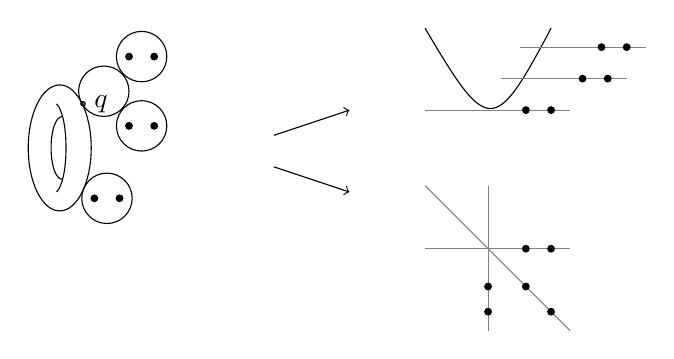
\begin{tikzpicture}[scale=.8]
\draw (-.1,0) circle (.4cm);
\draw[fill=gray] (-.43,-.20) circle[radius=1pt] node[right=.02cm]{$q$};
\draw (.5,.55) circle (.4cm);
\draw[fill=black] (.3,.55) circle[radius=1.5pt];
\draw[fill=black] (.7,.55) circle[radius=1.5pt];
%\node [above right] at (.8,.7) {$d_1$};
\draw (.5,-.55) circle (.4cm);
\draw[fill=black] (.3,-.55) circle[radius=1.5pt];
\draw[fill=black] (.7,-.55) circle[radius=1.5pt];
%\node [above right] at (.8,-.45) {$d_2$};
\draw (-.8,-.9) ellipse (.5cm and 1cm);
\draw (-.85,-.2) .. controls (-.65,-.4) and (-.65,-1.4) .. (-.85,-1.6);
\draw (-.75,-.4) .. controls (-1,-.4) and (-1,-1.4) .. (-.75,-1.4);
\draw (-.05,-1.7) circle (.4cm);
\draw[fill=black] (.15,-1.7) circle[radius=1.5pt];
\draw[fill=black] (-.25,-1.7) circle[radius=1.5pt];
%\node [above right] at (.25,-1.8) {$d_3$};

\draw[->] (2.6,-.7) -- (3.8,-.3);
\draw[->] (2.6,-1.2) -- (3.8,-1.6);

\draw[gray] (5,-.3)-- (7.3,-.3);
\draw[fill=black] (7,-.3) circle[radius=1.5pt];
\draw[fill=black] (6.6,-.3) circle[radius=1.5pt];
%\node [right] at (7,-.2) {$d_3$};
\draw (5,1) .. controls (6,-.7) and (6.1,-.7) .. (7,1);
\draw[gray] (6.5,.7)-- (8.5,.7);
\draw[fill=black] (7.8,.7) circle[radius=1.5pt];
\draw[fill=black] (8.2,.7) circle[radius=1.5pt];
%\node [right] at (8.5,.8) {$d_1$};
\draw[gray] (6.2,.2)-- (8.2,.2);
\draw[fill=black] (7.5,.2) circle[radius=1.5pt];
\draw[fill=black] (7.9,.2) circle[radius=1.5pt];
%\node [right] at (8.2,.3) {$d_2$};

\draw[gray] (5,-2.5)-- (7.3,-2.5);
\draw[fill=black] (7,-2.5) circle[radius=1.5pt];
\draw[fill=black] (6.6,-2.5) circle[radius=1.5pt];
%\node [right] at (7,-2.4) {$d_3$};
\draw[gray] (6,-1.5)-- (6,-3.8);
\draw[fill=black] (6,-3.5) circle[radius=1.5pt];
\draw[fill=black] (6,-3.1) circle[radius=1.5pt];
%\node [right] at (6.2,-1.5) {$d_2$};
\draw[gray] (5,-1.5)-- (7.3,-3.8);
\draw[fill=black] (7,-3.5) circle[radius=1.5pt];
\draw[fill=black] (6.6,-3.1) circle[radius=1.5pt];
%\node [right] at (7,-3.4) {$d_1$};
\end{tikzpicture}
\caption{Two different plausible $3$-stabilisations.}
\end{figure}
this curve is not $3$-stable. We could contract the maximal unpointed subcurve of genus one, but it is not balanced; on the other hand, say we could consistently contract the minimal genus one subcurve: by smoothing the node $q$ and doing so, we would get a family of $3$-fold elliptic points specialising to the tacnode, which can be excluded by studying the miniversal deformation of the latter. This problem is studied in \cite[\S 4.1]{SMY2}. \end{rmk}
I will discuss a specific variation on this \cite[Theorem 4.4]{BCM} that I am going to need later. Recall that $\mathfrak M_{1}^{\operatorname{wt}=d,\text{st}}$ is the open and bounded substack within the Artin stack of prestable curves with a weight assignment, defined by the conditions that the total weight is $d$ and the curve is weighted-stable; similarly $\mathfrak M_{1}^{\operatorname{wt}=d,\text{st}}(1)$ is the stack of weighted $1$-stable (at worst cuspidal) curves.
\begin{prop}\label{prop:1-stab}
There exists a morphism $\mathfrak M_{1}^{\operatorname{wt}=d,\text{st}}\to\mathfrak M_{1}^{\operatorname{wt}=d,\text{st}}(1)$ which extends the identity on the smooth locus.
\end{prop}

The proof is inspired by \cite[\S2]{HassettHyeon} and \cite[\S3.7]{RSPW}. We construct the contraction over $\MM_1^{\rm{div}}$ (the moduli space of nodal curves of genus one with a simple smooth divisor of total degree $d$ that makes them weighted-stable) first, and then show that it descends to $\MM_1^{\rm{wt,st}}$. We do so in order to have a natural polarisation.

Let $\pazocal E$ be the locus inside the universal curve over $\MM^{\rm{wt,st}}_1$ spanned by elliptic tails of weight $0$; this is a Cartier divisor, and abusing notation I will denote by $\pazocal E$ all its pullbacks. Moreover let $\mathfrak D^1$ be its image in $\MM^{\rm{wt,st}}_1$, which is a Cartier divisor as well.

Consider the following line bundle on the universal curve over $\MM_1^{\rm{div}}$: 
\begin{equation*}\label{eq:linebundlecontraction}
\mathcal N:=\omega_{\pi}(\pazocal E)\otimes\mathcal O_{\cC}(2\pazocal D),
\end{equation*} where $\pazocal D$ is the universal Cartier divisor over $\MM_1^{\rm{div}}$.

\begin{prop}\label{1-stabilization-div}
Let $\hC=\underline{\operatorname{Proj}}_{\MM_1^{\rm{div}}}(\bigoplus_{n\geq 0}\pi_*\mathcal N^{\otimes n})$. Then $\hC$ is a family of weighted $1$-stable curves and $\phi$ is a regular morphism:
 
 \bcd
 (\cC,\pazocal D)\ar[rr,"\phi"]\ar[dr,"\pi"] & & (\hC,\phi(\pazocal D))\ar[ld,"\bar{\pi}" above left] \\
 & \MM_1^{\rm{div}} &
 \ecd
This defines the $1$-stabilisation morphism $\MM_1^{\rm{div}}\to\MM_1^{\rm{div}}(1)$.
\end{prop}

Notice that $\mathcal N$ is trivial on the locus of elliptic tails, so this will be contracted by $\phi$. We need to prove that $\mathcal N$ is $\pi$-semiample (regularity of $\phi$) and that $\pi_*\mathcal N$ is locally free (flatness of $\bar{\pi}$). This is clear on the smooth locus; to prove it along $\mathfrak D^1$ we use \cite[Lemmma~3.7.2.2]{RSPW}.
\begin{lem}[Pullback with a boundary]\label{DVR}
Let $\pi\colon\cC\to S$ be a proper family of curves over a smooth basis, and let $\mathcal N$ be a line bundle on $\cC$ such that $\operatorname{R}^1\pi_*\mathcal N$ is a line bundle supported on a Cartier divisor $\mathfrak D\subseteq S$. Then for every DVR scheme $\dvr$ with closed point $0$ and generic point $\eta$, and for every morphism $f\colon \dvr\to S$ such that $f(0)\in\mathfrak D$ and $f(\eta)\in S\setminus\mathfrak D$ we have
\[f^*\pi_*\mathcal N\cong \pi_{\dvr,*}f_\cC^*\mathcal N.\]
\end{lem}

\begin{lem}\label{lemma:semiample}
The line bundle $\mathcal N$ is $\pi$-semi-ample, i.e. the natural map
\[\pi^*\pi_*\mathcal N^{\otimes n}\to \mathcal N^{\otimes n}\]
is surjective for $n\gg 0$.
\end{lem}
\begin{proof}
Outside the locus of elliptic tails $\mathcal N$ is $\pi$-ample. We are left with checking at points of an elliptic tail; thanks to the above Lemma we can reduce to the case that $C$ is the central fiber of a one-parameter smoothing with regular total space. The fact is then proved within Smyth's contraction lemma \cite[Lemma~2.12]{SMY1}.
\end{proof}

\begin{lem}
$\pi_*\mathcal N$ is locally free on $\MM_1^{\rm{div}}.$
\end{lem}
\begin{proof} Compare with \cite[Proposition~3.7.2.1]{RSPW}.
We check that $\pi_*\mathcal N$ has constant rank.
On $\MM_1^{\rm{div}}\setminus \mathfrak{D}^1$, $\operatorname{R}^1\pi_*\mathcal N=0$, so $\pi_*\mathcal N$ satisfies Cohomology and Base Change \cite[Theorem III.12.11]{HAR} and its rank is determined by Riemann-Roch, hence constant.
Given a point $x$ on the boundary $\mathfrak{D}^1$, we can pick a one-parameter smoothing as above, and we can check the rank at $x$ by looking at $\pi_*f^*\mathcal N$ over $\dvr.$ Now $f^*\mathcal N$ is flat over $\dvr$, so $\pi_*f^*\mathcal N$ is as well, which implies torsion-free and thus constant rank.
\end{proof}

\begin{proof}\eqref{1-stabilization-div}
Let $S\to \MM_1^{\rm{div}}$ be a smooth atlas, then we have:
 \bcd
 (\cC_S,\pazocal D_S)\ar[rr,"\phi_S"]\ar[dr,"\pi_S"] & & (\hC_S,\phi(\pazocal D_S))\ar[ld,"\bar{\pi}_S" above left] \\
 & S &
 \ecd
where $\hC_S=\underline{\operatorname{Proj}}_{S}(\bigoplus_{n\geq 0}\pi_{S,*}\mathcal N^{\otimes n})$, $\phi_S$ is a proper and birational, and $\bar{\pi}_S$ is a flat family. 
To verify that this defines a morphism $S\to \MM_1^{\rm{div}}(1)$ we have to argue that $\hC_S$ has reduced fibers and only nodes and cusps as singularities. After pulling back to a generic $\dvr$, this is again Smyth's contraction lemma \cite[Lemma~2.13]{SMY1}. $\mathcal D$ is pushed forward along $\phi$ and it satisfies weighted-stability, since $\phi$ is an isomorphism outside the locus of elliptic tails. To conclude that this defines a morphism $\MM_1^{\rm{div}}\to \MM_1^{\rm{div}}(1)$ it is enough to verify that there is an isomorphism
 $\rm{pr}_1^*\hC_S\cong\rm{pr}_2^*\hC_S$ satisfying the cocycle condition, where $\rm{pr}_i\colon S'= S\times_{\MM_1^{\rm{div}}} S\rightrightarrows S$.%and that $\rm{pr}_{ij}\colon S\times_{\MM_1^{\rm{div}}} S\times_{\MM_1^{\rm{div}}} S\to  S\times_{\MM_1^{\rm{div}}} S $ satisfy the cocycle condition.

 Now $\pr_i^*\hC_S$ is obtained by applying the Proj construction to 
 $\rm{pr}_i^*(\pi_{S,*}\mathcal{N})\cong\pi_ {S',*} (\rm{pr}_i^*\mathcal N)$, which are isomorphic because $S'\to S$ is flat. On the other hand $\rm{pr}_1^*\mathcal N\cong \rm{pr}_2^*\mathcal N$ since $\mathcal N$ is the pullback of a line bundle on $\MM_1^{\rm{div}}$. The cocycle condition is derived similarly. 
\end{proof}


\begin{lemma}
The $1$-stabilisation for curves with a divisor induces an analogous morphism at the level of weighted curves:
\bcd
\MM_1^{\rm{div}}\ar[r]\ar[d]\ar[dr,phantom,"\circlearrowright"] & \MM_1^{\rm{div}}(1)\ar[d] \\
\MM_1^{\rm{wt,st}}\ar[r,"\exists"] & \MM_1^{\rm{wt,st}}(1)
\ecd
\end{lemma}
\begin{proof}
{\'E}tale locally on $\MM_1^{\rm{wt,st}}$ we can choose smooth sections $s_i$ of the universal curve so that the Cartier divisor $\pazocal D=\sum s_i$ has degree compatible with the weight function, so in particular it makes $\mathcal N=\omega_{\pi}(\pazocal E)\otimes\mathcal O_{\cC}(2\pazocal D)$ trivial on the elliptic tails and $\pi$-ample elsewhere.
For a smooth atlas $S\to \MM_1^{\rm{wt,st}}$, this observation allows us to define a lifting $S\to \MM_1^{\rm{div}}$, and thus a morphism $\xi\colon S\to  \MM_1^{\rm{wt,st}}(1)$ via the construction of Proposition \ref{1-stabilization-div}.

In order to show that this descends to a morphism $\MM_1^{\rm{wt,st}}\rightarrow \MM_1^{\rm{wt,st}}(1)$ we need to verify that there exists $\rm{pr}_1^*(\xi)\cong\rm{pr}_2^*(\xi)$ satisfying the cocycle condition, where $\rm{pr}_i\colon S'= S\times_{\MM_1^{\rm{wt,st}}} S\rightrightarrows S$.

This boils down to checking that for two different choices of a lifting $\pazocal D_1,\pazocal D_2\colon S\to\MM_1^{\rm{div}}$ there exists a unique isomorphism 
\[\hC_1=\underline{\operatorname{Proj}}_S\left(\bigoplus_{n\geq 0}\pi_*(\mathcal N_1^{\otimes n})\right)\cong \underline{\operatorname{Proj}}_S\left(\bigoplus_{n\geq 0}\pi_*(\mathcal N_2^{\otimes n})\right)=\hC_2. \]
By construction there is a birational map $\psi$:
 \bcd
&\cC_S \ar[dl,"\phi_1" above left]\ar[dr,"\phi_2"]  \\
 \hC_1\ar[rr,dashed, "\psi"] & &\hC_2.
 \ecd

We want to show that $\psi$ extends to a regular morphism. 
Notice that $ \hC_i$ is normal, $i=1,2$: indeed since $S$ is smooth and the singularities of the fibers are in codimension $1$, $ \hC_i$ is regular in codimension $1$; since both $S$ (smooth) and the fibers (Cohen-Macaulay) satisfy Serre's condition $S_2$, so does the total space of $\hC_i$ by \cite[Thorem~23.9]{MAT}. By Zariski's connectedness theorem $\phi_{i,*}\OO_{\cC_S}\cong \OO_{\hC_i}$.
By construction $\operatorname{Exc}(\phi_1)=\operatorname{Exc}(\phi_2)$ is the locus of elliptic tails of weight $0$, so in particular $\phi_2$ contracts all the fibers of $\phi_1$. Then \cite[Lemma 1.15]{debarre}
implies that $\phi_2$ factors through $\phi_1$, and viceversa. This proves the regularity of $\psi$ and its inverse. Notice that $\psi$ is unique as it is the only extension of $\phi_2\circ\phi_1^{-1}$.
\end{proof} 

This concludes the proof of Proposition \ref{prop:1-stab}.

\subsection{Viscardi's moduli spaces of maps} I finally come to M. Viscardi's definition of alternative compactification of the space of maps from a smooth elliptic curve \cite[Definition 2.15]{VISC}.

\begin{dfn}
 The moduli space of $m$-stable maps $\oM^{(m)}_{1,n}(X,\beta)$ parametrises $f\colon (C,\mathbf p)\to X$ of class $\beta$ such that:\begin{enumerate}
                                                                                                                                      \item $C$ has only nodes and $l$-fold elliptic points as singularities, with $l\leq m$, $p_a(C)=1$ and $\mathbf{p}=(p_1,\ldots,p_n)$ are smooth and disjoint sections,
                                                                                                                                      \item if $E\subseteq C$ is a connected subcurve contracted by $f$, and $p_a(E)=1$, then its \emph{level} is \[\lvert \{i\in[n]:\ p_i\in E\}\rvert+\lvert E\cap \overline{C\setminus E}\rvert >m,\]
                                                                                                                                      \item $\lvert\Aut(C,f)\rvert<+\infty$.
                                                                                                                                     \end{enumerate}

\end{dfn}
The usual Behrend-Fantechi's construction \cite[Proposition 6.2]{BF} endows $\oM^{(m)}_{1,n}(X,\beta)$ of the usual dimension. Setting $m=0$ recovers the usual space of Kontsevich's stable maps.

\begin{prop}\cite[Theorem 3.6]{VISC}
 $\oM^{(m)}_{1,n}(X,\beta)$ is a proper DM stack of finite type over $\kk$.
\end{prop}
Checking the valuative criterion for properness goes as follows: assume the generic fiber is smooth (in general we may work componentwise on the generic fiber); we may first complete the family over $\dvr$ as an ordinary stable map. If $f$ contracts the core and it does not satisfy $m$-stability, we can make it into doing so by a sequence of operations: alternate between contracting the core to a Smyth's singularity and \emph{sprouting}, i.e. blowing up at markings or nodes along the core. Notice that more sprouting may be required in order for the map to descend to the singularity (see \cite[Remark 2.6]{BCM}). As anticipated, Viscardi's moduli space of $m$-stable maps to $\PP^N$ ``collapses'' the boundary components $D^k_1(\PP^N,d)$ for $k\leq m$ (the pointed case is subtler, as usual), hence the following result \cite[Corollary 5.10]{VISC}.
\begin{prop}
 There exists an $m_0=m_0(d,n)$ such that, for $m\geq m_0$, $\oM^{(m)}_{1,n}(\PP^N,d)$ is irreducible.
\end{prop}
\subsection{Aligned log structures} Finally, I would like to discuss how these two lines of thought (Li-Vakil-Zinger desingularisation and reduced invariants, compared to Smyth-Viscardi alternative compactifications) are not unrelated. A main issue with the Vakil-Zinger desingularisation is that the iterated blow-up procedure makes the modular interpretation of the resulting space not immediately clear. This has been fixed recently by D. Ranganathan, K. Santos-Parker and J. Wise with the introduction of the notion of an \emph{aligned} log curve. Recall the description of log smooth curves, due to F. Kato \cite{KatoF}, and the parallel with marked prestable curves. Let us work over a geometric point $S=\Spec(\kk=\bar\kk)$. In the genus one case, we can modify the usual dual graph construction by collapsing all the vertices corresponding to components of the core (in case the latter is a circle of $\PP^1$) to one vertex, called the \emph{circuit} and denoted by $\circ$. Define an $\oM_S$-valued function on the dual graph $\Gamma(C)$ by \[\lambda(v)=\sum_{e\in[\circ,v]}\rho_e,\] i.e. by associating to a vertex/component the sum of all the smoothing parameters of the edges/nodes separating it from the circuit.
\begin{dfn}
 Let $S$ be a log scheme and $C\to S$ a family of log smooth curves of genus one. We say that $C$ is \emph{radially aligned} if for every geometric point $s\in S$ the values of $\lambda(v)$ are \emph{comparable} in $\oM_{S,s}$ for every vertex $v$ of $\Gamma(C_s)$.
\end{dfn}
There exist \emph{minimal} radially aligned log structures, hence the moduli problem over $(LogSch)$ is the enhancement of a moduli stack over $(Sch)$ endowed with a log structure, after work of D. Gillam \cite{Gillam}. At this level
\[\MM^{\mathrm{rad}}_{1,n}\to\MM_{1,n}\]
is a log modification, due to the key observation that a log blow-up along a log ideal $K$ determines on every one of its charts a minimal element among the generators of $K$, hence a sequence of log blow-ups will serve the goal of ordering a collection of sections of $\oM_S$ \cite[Lemma 3.36]{Kelithesis}. Pictorially, it corresponds to a subdivision of the dual minimal monoid (see \cite[\S 3.3-3.4]{RSPW}). On the other hand, for every \emph{stable} radially aligned curve over a geometric point $S$, and for every integer $m\geq0$, we may find a section $\delta_m$ of $\oM_S$ such that $\delta_m=\lambda(v)$ for some vertex of $\Gamma(C)$, and the circle of radius $\delta_m$ has inner valence less than $m$ and outer valence strictly larger than $m$. $\delta_m$ behaves well under specialisation/generisation, by semicontinuity of the inner and outer valence \cite[Proposition 3.5.2]{RSPW}, hence it can be defined over any base. The power of log structures is two-fold at this point:
\begin{enumerate}
 \item it produces a log-modification $\widetilde{C}\to C$ by subdividing the edges where they meet the circle of radius $\delta_m$ (i.e. blowing up some nodes and markings on the components with $\lambda(v)<\delta_m$) \cite[Proposition 3.6.1]{RSPW};
 \item by combining $\lambda$ and $\delta_m$, it produces a $\tilde{\pi}$-semiample line bundle on $\widetilde{C}$, the morphism associated to which contracts the strict interior of the circle of radius $\delta_m$, producing a diagram as follows, with $\bar{\pi}\colon\overline{C}\to S$ an $m$-stable Smyth's curve \cite[Proposition 3.7.3.1]{RSPW}.
 \bcd[cramped]
 & \widetilde{C}\ar[dl]\ar[dr] & \\
 C\ar[dr,"\pi"] & & \overline{C}\ar[dl,"\bar{\pi}"] \\
 & S &
 \ecd
\end{enumerate}
\begin{rmk}
 It may seem that this construction sometimes happens to contract unbalanced curves, but it is not the case; notice that the blow-ups in point (1) above may occur along non-reduced centers. In fact, the strict interior of a circle around the circuit is the correct generalisation of a balanced elliptic tail when $C\to S$ is not just a one-parameter smoothing with regular total space.
\end{rmk}
This construction in the stable case provides a resolution of indeterminacy of the birational map between different Smyth's compactifications:
\bcd[cramped]
& \oM_{1,n}^{\mathrm{rad}}\ar[dr]\ar[dl] & \\
\oM_{1,n} \ar[rr,dashed] & & \oM_{1,n}^{(m)}
\ecd
More to the point, there is an important extension of this construction to the realm of maps.
\begin{dfn}
 A \emph{centrally aligned map} $f\colon(C,\mathbf p)\to X$ over $S$ is a log morphism (where $X$ has the trivial log structure) with a section $\delta_0$ of $\oM_S$, such that $\delta_0=\lambda(v)$ for $v$ of minimal distance to the circuit among the non-contracted components, $\lambda(w)$ is comparable with $\delta_0$ for every $w$, and the $\lambda(w)$ are comparable with one another whenever they are less than $\delta_0$.
\end{dfn}
The section $\delta_0$ together with $\lambda$ defines a modification $\widetilde{C}$ and a contraction to $\overline{C}$ with a Smyth's singularity as aboce.
\begin{dfn}
 A centrally aligned map satisfies the \emph{factorisation property} if its pullback to $\widetilde{C}$ descends to $\overline{C}$:
 \bcd[cramped]
 & \widetilde{C}\ar[dl]\ar[dr] & \\
 C\ar[dr,"f"] & & \overline{C}\ar[dl,dashed,"\exists\bar{f}"] \\
 & X &
 \ecd
\end{dfn}
\begin{thm}\cite[Theorems 4.6.3.2 and 4.5.1]{RSPW}
 The moduli space of centrally aligned maps to projective space is isomorphic to the Vakil-Zinger blow-up. The factorisation property identifies the main component.
\end{thm}
Notice that by construction $\bar{f}$ is non-constant on at least one branch of the core. For every Gorenstein curve of genus one with no separating nodes, the dualising sheaf is trivial \cite[Lemma 3.3]{SMY1}. Therefore $H^1(\overline{C},\bar{f}^*\OO_{\PP^N}(1))=0$ by Serre duality, and the projection to $\MM^{\mathrm{cen}}$ is unobstructed (a perfect obstruction theory is given by $\R\bar{\pi}_*\bar{f}^*T_{\PP^N}$), so every element satisfying factorisation is smoothable; on the other hand factorisation is a closed condition \cite[Theorem 4.3]{RSPW}. This proves the second claim above.

\begin{rmk}
 From the discussion above we see that the construction in \cite{RSPW} might be suitable to extend the definition of reduced invariants to a larger class of varieties than projective complete intersections. It would be enough that $\VZ{n}{X}{\beta}$ is irreducible and $Y\subseteq X$ is such that $N_{Y/X}$ is an ample vector bundle, so that $\operatorname R^1\bar{\pi}_*\bar{f}^*N_{Y/X}=0$ and the inclusion $\VZ{n}{Y}{\beta}\hookrightarrow\VZ{n}{X}{\beta}$ admits a perfect obstruction theory. On the other hand if we want to prove that $\VZ{n}{X}{\beta}$ is smooth following in the steps above, we need $T_X$ ample, which is quite a restrictive condition (the only smooth variety with ample tangent bundle is the projective space, by a theorem of Mori \cite{Mori}, on the other hand it could be possible e.g. to extend to the orbifold theory of weighted projective spaces).
\end{rmk}
\subsection{Reduced vs cuspidal invariants} In the next section I am going to discuss a result that I have obtained with F. Carocci and C. Manolache, which illustrates the relation between the Li-Vakil-Zinger's and the Smyth-Viscardi's projects under a slightly different light: namely, the idea is that the reduced invariants may be recovered as $m$-stable invariants, when $m$ is big enough that all the boundary components contributing non-trivially to the right hand side of the Li-Zinger's formula have been deleted. We demonstrate this principle in the case of the quintic threefold, for which only $D^1$ matters, so that it is enough to allow maps from cuspidal curves.

\begin{thm}\cite{BCM}\label{thm:redvscusp}
 For a smooth quintic threefold $X_5=V(\mathbf w)\subseteq \PP^4$, \[GW_1^{\mathrm{red}}(X_5)=GW_1^{(1)}(X_5).\]
\end{thm}
This is really a result about the virtual cycles, hence it holds for any (descendent) insertion. Here is an idea of how the proof could go: recall from Proposition \ref{prop:1-stab} that there is a well-defined $1$-stabilisation morphism at the level of weighted-stable curves; the following fiber product
\bcd
\mathcal Z_X\ar[r,"\alpha"]\ar[d]\ar[dr,phantom,"\Box"] & \oM^{(1)}(X_5,d)\ar[d] \\
\mathfrak M_{1}^{\operatorname{wt}=d,\text{st}}\ar[r] & \mathfrak M_{1}^{\operatorname{wt}=d,\text{st}}(1)
\ecd
is endowed with a class $\virt{\mathcal Z_X}$ by virtual pullback, such that $\alpha_*\virt{\mathcal Z_X}=\virt{\oM^{(1)}(X_5,d)}$, because $\mathfrak M_{1}^{\operatorname{wt}=d,\text{st}}\to \mathfrak M_{1}^{\operatorname{wt}=d,\text{st}}(1)$ is proper \cite[Lemma 4.19]{BCM} and birational, and by commutativity of virtual pullbacks with proper pushforward \cite{Manolache-Pull}. On the other hand there is a closed embedding of $\mathcal Z_X$ into ordinary stable maps $\oM_1(X,d)$ \cite[Lemma 4.13]{BCM}; it is an isomorphism with the substack of maps satisfying factorisation through $1$-stabilisation of the underlying weighted curve. In particular $\mathcal Z_X$ has a main component, and all the boundary components except $D^1(X,d)$. Unfortunately it is hard to study the intrinsic normal cone of $\oM_1(X,d)$ directly, hence we resort to an indirect approach, extending work of H.L. Chang, Y. Hu, Y.-H. Kiem and J. Li to the situation at hand.

\subsection{A word on genus two}

This section is based on discussions I have had with F. Carocci. The geometry of the moduli space of maps of genus two to $\PP^N$ is more complicated than that of genus one. A key focus of recent research has been towards verifying the \cite{BCOV} prediction for the higher genus Gromov-Witten potential (of the quintic threefold). Zinger managed to do so in genus one \cite{Zinger-CYhyp}, as the culmination of the articulate project I have tried to outline in the previous sections. An approach to the genus two case \`a la Li-Vakil-Zinger, i.e. through a partial desingularisation of the moduli space, has been attempted by Hu and Li in \cite{HL2}: it is quite subtle, even though incomplete, and it appears to have remained dormant for more than five years now. On the other hand there has been a recent breakthrough, due to S. Guo, F. Janda, and Y. Ruan \cite{GJR}, based on torus localisation on a compactification - inspired by the theory of log stable maps - of the moduli space of maps with $p$-fields (in fact of a more general GLSM moduli space \cite{CJRS}). Nonetheless I believe it would be relevant to gain a better understanding of the geometry of the moduli space of maps, possibly with a view towards the definition of reduced invariants, which should provide a modular definition of BPS numbers \cite{PandhaHodge}, at least under some extra hypotheses (e.g. the curve class is primitive).

Following Smyth's procedure in \cite[Appendix A]{SMY1}, we are able to classify the unibranch singularities of genus two. Let $(R,\m)$ be the completion of the local ring of the curve at the singularity, with normalisation:
\[(\tR,\tm)\simeq\left(\kk[\![t_1]\!]\oplus\ldots\oplus\kk[\![t_m]\!],\langle t_1,\ldots,t_m\rangle\right).\]
So $m$ is the number of branches, and $\delta=m+1$ for $g=2$ (compare with Definition \ref{def:genus}). It is an observation of Smyth that $\tR/R$ is graded by:
\[ (\tR/R)_i:=\tm^i/(\tm^i\cap R)+\tm^{i+1};\]
furthermore he notices that:
\begin{enumerate}
\item $m+1=\delta(p)=\sum_{i\geq 0}\dim_\kk(\tR/R)_i;$
\item $2=g=\sum_{i\geq 1}\dim_\kk(\tR/R)_i;$
\item if $(\tR/R)_i=(\tR/R)_j=0$ then $(\tR/R)_{i+j}=0$.
\end{enumerate}
The following facts will also turn out to be useful:
\begin{enumerate}[resume]
 \item $\sum_{i\geq k}(\tR/R)_i$ is a grading of $\tm^k/(\tm^k\cap R)$;
 \item there is an exact sequence:
 \[ 0\to \frac{\tm^k\cap R}{\tm^{k+1}\cap R}\to \frac{\tm^k}{\tm^{k+1}}\to \left(\tR/R\right)_k\to 0.\]
\end{enumerate}

Notice that in the unibranch case $\dim_\kk(\tR/R)_1\leq 1$, hence equality must hold (by observation (3) above). We are thus left with two cases:
 \begin{enumerate}
  \item either $\dim_\kk(\tR/R)_2=1$ and $\dim_\kk(\tR/R)_i=0$ for all $i\geq 3$: in this case $\tm^3\subseteq\m$ by observation (4). Indeed we see by (5) that \[\tm^3=\m,\] hence $R\simeq\kk[\![t^3,t^4,t^5]\!],$ a non-Gorenstein singularity.
  
  \item or $\dim_\kk(\tR/R)_3=1$ and $\dim_\kk(\tR/R)_i=0$ for $i=2$ and for all $i\geq 4$: in this case $\tm^4\subseteq\m$ by observation (4). On the other hand from $\dim_\kk(\tm^2\cap R/\tm^3\cap R)=1$ we deduce that there is a generator of degree $2$, and from $\dim_\kk(\tm^3\cap R/\tm^4\cap R)=0$ there is none of degree $3$; so we see that \[\m/\m^2=\langle t^2,t^5\rangle,\] i.e. $R\simeq\kk[\![x,y]\!]/(x^5-y^2)$, which is planar (hence Gorenstein).
 \end{enumerate}

We can show that the semistable models are as follows:
 \begin{enumerate}
  \item the non-Gorenstein singularity is obtained by collapsing a genus two tail which is attached to a rational tree at a non-Weierstrass point;
  \item the planar singularity is obtained by collapsing a genus two tail which is attached to a rational tree at a Weierstrass point.
 \end{enumerate}
The idea is again that the normal surface you get after contracting is Gorenstein if and only if it has Gorenstein central fiber, if and only if the line bundle used to perform the contraction may be written as $\omega_{\mathcal C}(D)$ with $D$ supported on the exceptional locus, and such that $\omega_{\mathcal C}(D)_{|\operatorname{Exc}(\phi)}$ is trivial.

\begin{rmk}
 It was pointed out by D.I. Smyth that we cannot always construct simultaneous smoothings of the singularity and a semistable curve mapping to it (compare with \cite[Lemma 2.11]{BCM}). In particular it will not be true that any map that factors through a genus two singularity (and does not contract all of its branches) is automatically smoothable. Consider the map $f_0\colon\PP^1\to\PP^3$ given in coordinates by \[ [s:t]\mapsto[s^3t^2:t^5:st^4:s^5].\]
 It is the normalisation of a curve with a singularity of type (2) above. Now attach a genus two curve with a non-Weierstrass point to $(\PP^1_{[s:t]},[1,0])$, and let it be collapsed by the map. Assume the resulting genus two stable map were smoothable: then, by pulling back $\OO_{\PP^3}(1)$ and taking the relative Proj construction, we would get a family $\overline{\mathcal C}$ with central fiber of type (1), and such that the map $f\colon\mathcal C\to\PP^3$ factors through $\overline{\mathcal C}$. But this map should restrict to an isomorphism of the central fiber with its image (because the map is birational, and the two curves have same normalisation and $\delta$-invariant), which is a contradiction.
\end{rmk}

\begin{rmk}
 There are a number of genus two singularities with two branches. The complexity of carrying out an algebraic study as above increases steeply with the number of branches. On the other hand every genus two singularity with two branches is obtained by gluing two singularities $R_1$ and $R_2$ with $g(R_i)\leq 2$ along a closed subscheme of length $\leq 3$.
 This is clear if we look at the factorisation of the normalisation $R\hookrightarrow \widetilde{R}=k[\![t_1]\!]\oplus k[\![t_2]\!]$ through $R\hookrightarrow R_1\oplus R_2\hookrightarrow \widetilde{R},$ where 
 the first partial normalisation corresponds to separating the branches. Algebraically, this can be achieved by considering the quotient $K^{\rm{br}}$ of $\widetilde{R}/R$ generated by those conditions involving only one branch at the time, and then taking the kernel of $\widetilde{R}\to K^{\rm{br}}.$ For example $\kk[\![x,y]\!]/(y(x^3-y))$ is obtained by gluing two smooth branches. Compare with \cite[Appendix A]{SMYtowards}.
\end{rmk}

Finally, the components of $\M{2}{n}{\PP^N}{d}$ are included in the following list (I will not mention the various possible distributions of the markings, and I will represent the decorated dual graph of a general element of each component):
\begin{enumerate}
 \item the main component is the closure of the locus of maps from a smooth curve of genus two;
 \item $\mathcal D^k=\left\{\Dk\right\}$
  \item $\mathcal D^{\rm{hypell},k}=\left\{\hypell\right\}$
 \item $\mathcal E^k=\left\{\Ek\right\}$
 \item $\mathcal E^{(k_1,k_2)}=\left\{\Ekk\right\}$
 \item $\mathcal E^{\rm{nct}}=\left\{\pacman\right\}$
\end{enumerate}
Here is a funny example: consider $\oM_2(\PP^1,3)$. From the theory of limit linear series, no element of $\mathcal D^{\rm{hypell},1}$ is smoothable: let the underlying curve be $Z\coprod_q R$, where $Z$ has genus two and $R\simeq\PP^1$. The aspect supported on $Z$ is $\omega_Z(q)$, with vanishing sequence $(1,3)$ (if $q$ Weierstrass) and $(1,2)$ (otherwise), so the aspect $\mathcal L$ supported on $R$ has vanishing sequence $(0,2)$ or $(1,2)$; in any case $\mathcal L(-2Z)$ has only one section, so it cannot give a map to $\PP^1$. On the other hand $\mathcal D^{\rm{hypell},1}$ intersects $\mathcal D^2$, $\mathcal D^3$, $\mathcal E^1$, $\mathcal E^{0,1}$, $\mathcal E^{0,2}$, and $\mathcal E^{1,1}$. 

\section{p-fields, local equations and a splitting of the cone}

The indirect approach to the proof of Theorem \ref{thm:redvscusp} can be outlined as follows: we introduce the moduli space of $1$-stable maps with $p$-fields, $\oM_1^{(1)}(\PP^4,d)^p$, the geometry of which is closely related to that of $\oM_1^{(1)}(\PP^4,d)$ (in fact, it is a line bundle over the boundary, while the open main components are isomorphic); $\oM_1^{(1)}(\PP^4,d)^p$ is endowed with a cosection localised virtual class carrying the same information as $\virt{\oM_1^{(1)}(X,d)}$. By pulling back along the $1$-stabilisation as above, we may define $\mathcal Z_{\PP^4}$ and $\mathcal Z^p$; unfortunately $\mathcal Z^p$ does not compare directly with $\oM_1(\PP^4,d)^p$. On the other hand, after studying local equations for the moduli space and a Vakil-Zinger blow-up, we are able to split the normal cone of $\tZp$ directly, and show that the only non-trivial contribution to the invariants comes from the main component.

\subsection{$1$-stable maps with $p$-fields} In \cite{CLpfields}, Chang and Li develop a general theory of moduli spaces of sections: let us work over a base $B$ - an algebraic stack - and let $\pi\colon \cC\to B$ be a family of proper l.c.i. curves (they restrict to the nodal case, but all their arguments carry through unchanged, as we have checked in \cite[\S 3]{BCM}). Let $\mathcal V$ be representable, quasi-projective, and smooth over $\cC$. The \emph{space of sections} of $\mathcal V$ over $\cC$ is a $B$-stack $\mathfrak S$ defined by:
 \[\mathfrak{S}(S\to B)=\left\{\text{sections of}\ \mathcal V_S\to\cC_S\right\};\]
it has a dual perfect obstruction theory relative to $B$ \cite[Proposition 2.5]{CLpfields}:
\[ \phi_{\mathfrak S/B}\colon T^{\bullet}_{\mathfrak S/B}\to E^{\bullet}_{\mathfrak S/B}:=\R\pi_{\mathfrak S,*}\mathfrak e^* T_{\mathcal V/\cC}.\]
This applies in particular when $\mathcal V$ is a vector bundle over $\mathcal C$ (or an open within one), and in this case we get a \emph{cone} of sections $C(\mathcal V)$; in fact by Serre duality \[C(\mathcal V)=\underline{\Spec}_B\operatorname{Sym}^\bullet(\operatorname{R}^1\pi_* (V^\vee\otimes \omega_{\mathcal C/B})).\] If we let $B=\mathfrak{P}$ be the universal Picard stack over $\MM$, we recover the moduli space of stable maps to $\PP^N$ as an open (defined by stability and the fact that the section do not vanish simultaneously) inside $C(\pi_*(\mathcal L)^{\oplus N+1})$; the relative obstruction theory $\R\pi_*\mathcal L^{\oplus N+1}$ over $\mathfrak{P}$ is compatible with the usual one $\R\pi_*f^*T_{\PP^N}$  over $\MM$, by the Euler sequence and $T^{\bullet}_{\mathfrak P/\MM}\simeq\R\pi_*\OO_{\mathcal C}[1]$ \cite[Lemma 2.8]{CLpfields}. This is familiar from the theory of quasimaps (it is just a change in the stability condition cutting a different open within the Artin stack of sections).
\begin{dfn}
 The moduli space of $1$-stable maps with $p$-fields $\oM_1^{(1)}(\PP^4,d)^p$ parametrises $1$-stable maps $\bar{f}\colon\overline{C}\to\PP^4$ together with a \emph{$p$-field}: \[\psi \in  H^0(\overline{C},\bar{f}^*\OO_{\PP^4}(-5)\otimes\omega_{\bar{\pi}}).\]
\end{dfn}
 \noindent It is the cone of sections of the line bundle $\overline{\mathcal P}=\bar{f}^*\OO_{\PP^4}(-5)\otimes\omega_{\bar{\pi}}$ over $\oM_1^{(1)}(\PP^4,d)$. Notice that it is isomorphic to $\oM_1^{(1)}(\PP^4,d)$ on the open locus of the main component, while it is a line bundle over the boundary components; in particular it is not a proper space. It has a perfect obstruction theory relative to $\overline{\mathfrak P}=\mathfrak{Pic}(\overline{\mathcal C}\to\MM_1(1))$ given by $\R\bar{\pi}_*(\overline{\mathcal L}^{\oplus 5}\oplus \overline{\mathcal P}),$
 where $\overline{\mathcal P}$ is defined as above replacing $\bar{f}^*\OO_{\PP^4}(1)$ by the universal line bundle $\overline{\mathcal L}$.

The quintic polynomial $\mathbf w$ determines a cosection of the obstruction bundle as follows: there is a morphism of vector bundles on the universal curve over $\hP$:
$ h_1\colon\rm{Vb}(\hL^{\oplus 5}\oplus\overline{\mathcal P})\to \rm{Vb}(\omega_{\bar\pi}),\quad h_1(\mathbf{x},p)=p\w(x_0,\ldots,x_4).$
By differentiating it and pulling it back along the universal evaluation
\bcd
& \rm{Vb}(\hL^{\oplus 5})\setminus\{0\}\oplus\rm{Vb}(\overline{\mathcal P})\ar[d] \\
\hC\ar[ru,bend left,start anchor=north, end anchor=west,"\mathfrak e"]\ar[d,"\bar\pi"]\ar[r] & \hC\ar[d,"\bar\pi"] \\
 \oM_1^{(1)}(\PP^4,d)^p\ar[r] & \rm \hP
\ecd
%here and in future $\oplus$ at the level of geometric vector bundles means the fiber product over the base
 we obtain a cosection of the relative obstruction sheaf
\begin{multline}\label{eqn:cosection}
 \sigma_1\colon\rm{Ob}_{\oM_1^{(1)}(\PP^4,d)^p/\hP}=\operatorname{R}^1\bar\pi_*(\hL^{\oplus 5}\oplus\overline{\mathcal P})\to \operatorname{R}^1\bar\pi_*(\omega_{\bar\pi})\simeq \OO_{\oM_1^{(1)}(\PP^4,d)^p} \\
 \sigma_{1|(u,\psi)}(\mathring{\mathbf{x}},\mathring{p})=\mathring{p}\w(u)+\psi\sum_{i=0}^4\partial_i\w(u)\mathring{x}_i
\end{multline}

The degeneracy locus of this cosection is precisely $\oM_1^{(1)}(X,d)$ by Serre duality and smoothness of $X$. We may therefore apply Kiem-Li's machinery of cosection-localised virtual cycles \cite{KL}\cite[\S 5]{CLpfields}, to obtain a class supported on the degeneracy locus of $\sigma_1$: \[\virloc{\oM_1^{(1)}(\PP^4,d)^p}=0^{!}_{\sigma_1,\rm{loc}}[\mathfrak{C}_{\oM_1^{(1)}(\PP^4,d)^p/\hP}]\;\in\; A_0\left(\oM_1^{(1)}(X,d)\right).\] 

\begin{thm}\label{thm:p-fields-quintic}
 \[\deg[\Mone{1}{\PP^4}{d}^p]^{\rm{vir}}_{\rm{loc}}= (-1)^{5d}\deg[\oM_1^{(1)}(X,d)]^{\rm{vir}}\]
\end{thm}
This is proved by deforming to the normal cone and then working out explicitly the localised virtual pullback along $\oM_1^{(1)}(N_{X/\PP^4},d)^p\to \oM_1^{(1)}(X,d)$, which has a symmetric obstruction theory. All the details are spelled out in \cite{CLpfields} and summarised in \cite[\S 3]{BCM}.
\subsection{Auxiliary spaces} Consider now the fiber diagram:
\bcd
\mathcal Z^p \ar[r]\ar[d]\ar[rd,phantom,"\Box"] & \overline{\mathcal M}_1^{(1)}(\PP^4,d)^p \ar[d] \\
\XP \ar[r]\ar[d]\ar[rd,phantom,"\Box"] & \overline{\mathfrak{P}} \ar[d] \\
\MM_1^{\rm{wt,st}}\ar[r] & \MM_1^{\rm{wt,st}}(1)
\ecd

\begin{rmk}\label{rmk:Zp}
The stack $\XP$ parametrises $\cC\to \hC$ with a line bundle $\hL$ on $\hC$. By pulling back $\hL$ to $\cC$ we obtain a morphism $\XP\to \mathfrak{P}$. This is generically an isomorphism, but has $1$-dimensional fibers over the locus of elliptic tails, due to the fact that $\Pic(\overline{C})\to\Pic(C)$ has kernel $\mathbb G_{\rm a}$ when $\overline{C}$ has a cusp; on the other hand the line bundle thus obtained is always trivial on the elliptic tail, therefore $\XP\to \mathfrak{P}$ is not surjective, as it misses the non-trivial line bundles of degree $0$ on elliptic tails.

Similarly the stack $\mathcal Z^p$ parametrises $C\xrightarrow{\phi}\overline{C}\xrightarrow{\bar{f}} \PP^4$ with a $p$-field $\psi\in H^0(\hC_S,f_S^*\OO_{\PP^4}(-5)\otimes\omega_{\bar\pi_S})$. We were not able to compare $\Zp$ with $\oM_1(\PP^4,d)^p$ directly, since denoting by $\hL=f^*\OO_{\PP^4}(1)$ and by $\mathcal L=\phi^*\hL$ we only have a map $\operatorname{R}^1\bar\pi_*\hL\to\operatorname{R}^1\pi_*\mathcal L$ on $\Zp$ which is not an isomorphism.
\end{rmk}

$\mathcal Z^p$ is endowed with a localised virtual cycle that has the same degree as $[\Mone{1}{\PP^4}{d}^p]^{\rm{vir}}_{\rm{loc}}$, by commutativity of localised virtual pullback with proper pushforward \cite[Lemma 4.17]{BCM}.

\subsection{Local equations} In order to study the intrinsic cone of $\Zp$ we need to embed it, at least locally, in a smooth space, and understand the equations of the embedding. Since locally $\Zp$ sits inside $\mathcal Z_{\PP^4}\times \Aaff^1$, it is enough to find local equations for $\mathcal Z_{\PP^4}$. Recall that $\mathcal Z_{\PP^4}$ is an open inside the cone of sections $\bar{\pi}_*\hL^{\oplus 5}$ over $\hP$. It is standard to resolve $\R\bar{\pi}_*\hL$ twisting by a sufficiently $\bar{\pi}$-ample line bundle on $\hC$, but in the genus one case this can be performed very efficiently by twisting with a local section $\mathcal A$ passing through the core (a line bundle of positive degree on a Gorenstein genus one curve has no $h^1$); $\bar{\pi}_*\hL$ is then the kernel of the restriction map $\bar{\pi}_*\hL(\mathcal A)\to \bar{\pi}_*\hL(\mathcal A)_{|\mathcal A}$. Furthermore this map can be expressed very explicitly in local coordinates.

For technical reasons we work over $\mathfrak Z^{\rm{div}}:=\mathfrak Z\times_{\MM_1(1)}\MM_1^{\textrm{div}}(1)$: locally on $\mathcal Z_{\PP^4}$ we can choose a hyperplane $H_0\subseteq\PP^4$ that pulls back to a simple divisor contained in the smooth locus of the curve, say $D=\sum_{i=1}^d \delta_i$, and choose coordinates on $\PP^4$ such that $H_0=\{x_0=0\}$. Locally we thus get a map $\mathcal Z_{\PP^4}\to \mathfrak Z^{\rm{div}}$ by associating $(C\to\overline{C}\supseteq D=\bar{f}^{-1}(H_0))$ to $(C\to \overline{C}\xrightarrow{\bar{f}}\PP^4)$. By choosing a distinct local section $\mathcal B$ through the core, and by possibly restricting the chart $\mathcal U\to\mathcal Z_{\PP^4}$ we may write:
\begin{enumerate}
 \item $\bar{\pi}_*\hL=\bar{\pi}_*\hL(-\mathcal B)\oplus\OO_{\mathcal U}$,
 \item $\bar{\pi}_*\hL(-\mathcal B)=\operatorname{Ker}\left(\bar{\pi}_*\hL(\mathcal A-\mathcal B)\xrightarrow{\rm{res}_{\mathcal A}}\bar{\pi}_*\OO_{\mathcal A}(\mathcal A)\right)$, and
 \item $\bar{\pi}_*\hL(\mathcal A-\mathcal B)=\bigoplus_{i=1}^d \bar{\pi}_*\OO_{\overline{\mathcal C}}(\delta_i+\mathcal A-\mathcal B)\xrightarrow{\oplus \rm{res}^i_{\mathcal A}}\bar{\pi}_*\OO_{\mathcal A}(\mathcal A)$.
\end{enumerate}

Let me introduce some notation: around a point $[\overline{C}]\in\MM_1^{\rm{wt,st}}(1)$, for every node $q$ of $\overline{C}$ there is a coordinate $\zeta_q$ on $\MM_1$ whose vanishing locus is the divisor where that node persists. Denote by $\zeta_{[\delta_i,\pazocal A]}=\prod\zeta_q$
where the product runs over all the nodes separating $\delta_i$ from the core.
 
\begin{prop}\cite[Proposition 4.13]{HL}\label{prop:res}
The line bundles $\bar\pi_*\OO_{\overline{\mathcal C}}(\pazocal \delta_i+\A-\B)$ and $\bar\pi_*\OO_{\A}(\A) $ admit trivialisations such that:
\[\rm{res}^i_{\mathcal A}=\zeta_{[\delta_i,\A]}.\]
\end{prop}
\begin{prop}\label{prop:equations} \cite[Theorems 2.17-19]{HL}
A local chart $\pazocal U$ for $\mathcal Z_{\PP^4}$ can be embedded as an open inside:
\[ (F_0=\ldots=F_4=0)\subseteq \operatorname{Vb}_{\hP}(\bar{\pi}_*\hL(\A)^{\oplus 5}),\qquad F_j:=\sum_{i=1}^d \zeta_{[\delta_i,\pazocal A]}w_i^j \]
where $w_i^j$ are coordinates on the fiber of the $j$-th copy of $\rm{Vb}(\bar{\pi}_*\hL(\A))$ over (a chart of) $\hP$.
\end{prop}
The local equations and the method adopted to find them is essentially the same as in the case of stable maps \cite{HL}, except that there is no boundary component $D^1(\PP^4,d)$ in the $1$-stable case. Local equations can be used to give a proof of Vakil's criterion of smoothability (see Proposition \ref{prop:components}(2)), that I will include here.
\begin{proof}
 Let me start with the easiest degenerate situation: a contracted elliptic curve attached to a $\PP^1$ of degree $d$ at a single node $q$. Equations for the moduli space of maps around such a point look like: 
 \[\zeta_q\sum_{i=1}^d w_i^j=0,\;\;\;\text{for} \;\;\;j=1,\ldots,r.\]
 
 
  Thi point corresponds to a smoothable map if and only if the equations admit a solution with $\zeta_q\neq 0$, that is $\sum_{i=1}^d w_i^j=0$ for every $j$. Taking a coordinate $z$ on  $\PP^1$ centred at the node $q$,   the $i$-th basis vector corresponds to a polynomial vanishing at $q$ and at $\delta_l,\;\forall l\neq i$. This can be written as:
  \[e_i(z)=z\prod_{l\neq i}\frac{(z-\delta_l)}{-\delta_l},\] 
  where we have chosen a convenient normalisation. So the restriction to the rational tail of the map corresponding to the point of coordinates $(w_i^j)_{i=1,\ldots,d}^{j=1,\ldots,N}$ can be written as:
  \[[1:\sum_{i=1}^d w_i^1e_i(z):\ldots:\sum_{i=1}^d w_i^Ne_i(z)].\] 
  Differentiating with respect to $z$ we see that the image of the tangent vector at $q$ is given in affine coordinates around $f(E)$ by:
  \[(\sum_{i=1}^d w_i^1,\ldots,\sum_{i=1}^d w_i^N).\] 
  Hence smoothability is equivalent to the image of the tangent vector being zero.
 
 More generally we may assume that the dual graph is terminally weighted \cite[\S 3.1]{HL}. Assume there are $k$  rational tails of positive weight $R_h,\ h=1,\ldots,k$. Denote by $D(h)$ the set of indices $i$ such that $\delta_i$ belongs to the $R_h$, and by $E(h)$ the set of nodes separating the core from $R_h$. The equations will then take the following form:
 \[\sum_{h=1}^k\left(\prod_{q\in E(h)}\zeta_q\right)\left(\sum_{i\in D(h)}w_i^j\right)=0,\ j=1,\ldots,r,\]
 which can be assembled in matrix form as follows:
 $$W\cdot\underline\zeta:=\left(\sum_{i\in D(h)}w_i^j\right)_{j,h}\cdot\left(\prod_{q\in E(h)}\zeta_q\right)_h=0.$$
 We see that smoothability is equivalent to the linear dependence of the rows of the above matrix $W$. On the other hand we can choose a suitable coordinate $z_h$ around the node $q_h$ on $R_h$ and write the map as: 
 \[[1:p_h^1(z_h):\ldots:p_h^N(z_h)],\]
  where: 
 \[p_h^j(z_h)=\sum_{i\in D(h)}w_i^je_i^h(z_h) \quad \text{and} \quad e_i^h(z_h)=z_h\prod_{l\in D(h)\setminus\{i\}}\frac{(z_h-\delta_l)}{-\delta_l}.\] The elliptic curve is contracted to the point $[1:0:\ldots:0]$ and the tangent vector to $R_h$ at $q_h$ is mapped to the $h$-th row of $W$ (in affine coordinates around $f(E)$). Again we see that the map is smoothable if and only if the image of the tangent vectors to the rational tails at the nodes are linearly dependent in $T_{f(E)}\PP^N$.
 \end{proof}

\subsection{A Vakil-Zinger blow-up}
At this point we perform a modular blow-up of $\MM_1^{\rm{wt,st}}(1)$: we successively blow $\overline{\Theta}_k$ up, $k\geq 2$, that is the closure of the locus where the core has weight $0$ and there are $k$ rational tails of positive weight. After the $k$-th blow-up, the strict transform of $\overline{\Theta}_{k+1}$ is smooth, so the final result  $\widetilde{\MM}_1^{\rm{wt,st}}(1)$ is smooth as well. 

The fiber product 
\[\widetilde{\MM}_1^{\rm{wt,st}}(1)\times_{\MM_1^{\rm{wt,st}}(1)}\MM_1^{\rm{wt,st}}\]
recovers the Hu-Li blow-up $\widetilde{\MM}_1^{\rm{wt,st}}$. Indeed $\Theta_1$ is already a Cartier divisor in $\MM_1^{\rm{wt,st}}$, and the inverse image of $\overline{\Theta}_k$ is precisely $\Theta_k$; 
using the universal property of the blow-up, it can be shown that there are maps in both directions, and they are inverse to one another. 

After blowing up, the equations above are simplified and assume the following form:
\begin{equation}\label{eqn:VZblowup}\tilde\zeta\tilde w^j=0,\quad j=0,\ldots,4\end{equation}
where $\{\tilde\zeta=0\}$ is one of the newly created boundary divisors $\widetilde{\Theta}_k$ in $\widetilde{\MM}_1^{\rm{wt,st}}(1)$ (i.e. one of the exceptional divisors produced by the blow-up process), and $\tilde w$ is a suitably defined coordinate on the fiber of $\rm{Vb}(\bar{\pi}_*\hL(\A))$.


Summing up, we get:
\bcd
   &  \widetilde{\mathcal Z}^p \ar[r]\ar[d]\ar[rd,phantom,"\Box"] & \tM_1^{(1)}(\PP^4,d)^p \ar[d] \\
\tM_1(\PP^4,d)\ar[d] & \widetilde{\mathcal Z}_{\PP^4} \arrow[left hook->,swap]{l}{i}\ar[r]\ar[d]\ar[rd,phantom,"\Box"] & \tM_1^{(1)}(\PP^4,d) \ar[d] \\
\widetilde{\mathfrak{Pic}}_1\ar[d] &\widetilde{\XP}\ar[l]\ar[r]\ar[d]\ar[rd,phantom,"\Box"] & \widetilde{\mathfrak{Pic}}_1 (1)\ar[d]\\
\widetilde{\MM}^{\rm{wt,st}}_1 & \widetilde{\MM}^{\rm{wt,st}}_1\ar[equal]{l}\ar[r] & \widetilde{\MM}_1^{\rm{wt,st}}(1)
\ecd

Notice that the components of $\tZp$ are in bijection with those of $\Zp$, however all the boundary ones have the same dimension $5d+4$, and their intersection with main is a divisor in the latter.
The blow-up procedure does not affect the invariants:
\begin{lem}\label{lem:tilding}\cite[Proposition~2.5]{CL}
We have the identity:
\[\deg\virloc{\tZp}=\deg\virloc{\Zp}.\]
\end{lem}

\subsection{Splitting the cone} The restriction of the intrinsic cone to the open strata is easily understood, see \cite[Lemma 4.3]{CLpfields}. Recall that $\tZp\to\tXP$ has a dual perfect obstruction theory $E^{\bullet}_{\tZp/\tXP}=\R\bar\pi_*(\hL^{\oplus 5}\oplus\overline{\mathcal P})=:E^{\bullet}_1\oplus E^{\bullet}_2$.
\begin{lem}\label{lem:open_cones}
The intrinsic normal cone $\mathfrak{C}_{\tZp/\tXP}$ has the following properties:
\begin{enumerate}
\item Its restriction to the open $\tZ^{p,\circ}= \tZ^{p,\rm{main}}\setminus \bigcup_{k\geq 2}D^k \tZp$ is the zero section of $h^1/h^0(E^{\bullet}_{\tZp/\tXP})\rvert_{\tZ^{p,\circ}}$.
\item Its restriction to the open $\tZ^{p,\rm{gst},\circ}=\tZp - \tZ^{p,\rm{main}}$  is a rank $2$ subbundle stack of $h^1/h^0(E^{\bullet}_{\tZp/\tXP})\rvert_{\tZ^{p,\rm{gst},\circ}}$.
\end{enumerate}
\end{lem}
\begin{proof}\begin{enumerate}[leftmargin=.8cm]
\item Observe that $\tZ^{p,\circ}\cong \tZ^{\circ}$ because here $H^0(\overline{C}, \overline{L}^{\otimes -5}\otimes \omega_{\overline{C}})=0$. Moreover $\tZ^{\circ}$ is unobstructed on its image, which is an open of $\tXP$, because $\operatorname{R}^1\bar{\pi}_*\hL=0$.
So the normal cone is $[\tZ^{p,\circ}/\bar{\pi}_*\hL^{\oplus 5}_{\rvert\tZ^{p,\circ}}]$, which is the zero section of $h^1/h^0(E^{\bullet}_{\tZp/\tXP})\rvert_{\tZ^{p,\circ}}=[0\oplus \operatorname{R}^1\bar{\pi}_*\widehat{\mathcal P}/\bar{\pi}_*\hL^{\oplus 5}\oplus 0]\rvert_{\tZ^{p,\circ}}$.

\item We know that $\tZ^{p,\rm{gst},\circ}$ is a line bundle over $\tZ^{\rm{gst},\circ}$. From equation \ref{eqn:VZblowup} we see that the latter is smooth over its image $\pazocal W$ in $\tXP$, which is the codimension $2$ locus where the core has weight $0$, the line bundle is trivial on it, and there are at least two rational tails of positive degree. Recall that every smooth morphism $A\to B$ of relative dimension $n$ factors as $A\xrightarrow{\acute{e}t} B\times \Aaff^n\xrightarrow{\pr_1} B$. So we have
\bcd
\tZ^{p,\rm{gst},\circ} \ar[r,"\acute{e}t"] & \pazocal W\times\Aaff^{5d+6}\ar[r,hook]\ar[d,"q"] & \tXP\times \Aaff^{5d+6}\ar[d] \\
& \pazocal W \ar[r,hook] & \tXP
\ecd
where the bottom horizontal arrow is a codimension $2$ regular embedding. Thus 
\[\mathfrak{C}_{\tZp/\tXP}\rvert_{\tZ^{p,\rm{gst},\circ}}\cong \left[ q^* N_{\pazocal W/\tXP}/ \bar{\pi}_*\hL^{\oplus 5}\oplus\bar{\pi}_*\overline{\mathcal P}\right]\]
is a rank $2-(5d+6)$ subbundle stack of  $h^1/h^0(\mathbb E_{\tZp/\tXP})\rvert_{\tZ^{p,\rm{gst},\circ}}.$
\end{enumerate}
\end{proof}
Notice that the image of $\tZ^{\circ}$ in $\tM_1(\PP^4)$ contains $\tM_1(\PP^4)^{\rm{main}}\cap \widetilde{D}^1(\PP^4).$

Recall the definition of the \emph{closure of the zero section of a vector bundle stack}: let $B$ be an integral algebraic stack and let $F^{\bullet}=[F_0\xrightarrow{d} F_1]$ be a complex of locally free sheaves on $B$. The zero section is $0_{F^{\bullet}}\colon [F_0/F_0]\to h^1/h^0(F^{\bullet})=[F_1/F_0]$, which is in general not a closed embedding; its closure is defined as:
\[ \overline{0}_{F^{\bullet}}=[\overline{dF_0}/F_0]. \]
$\overline{0}_{F^{\bullet}}$ is an integral stack.

\begin{ex}
When $h^0(F^{\bullet})=0$, the closure of the zero section looks like $B$ with some further stacky structure on the vanishing locus of $d$. Consider for example $B=\PP^1$ and $F^{\bullet}=[\OO_{\PP^1}\xrightarrow{x}\OO_{\PP^1}(1)]$. Then the action of $e\in F_0$ on $F_1$ is given by $f\mapsto f+xe$. Clearly $\overline{dF_0}$ is the whole line bundle $F_1$; the $F_0$-action is transitive on the fibers over $\{x\neq 0\}$ and trivial on the fiber over $0$. Hence $\overline{0}_{F^{\bullet}}$ is isomorphic to $\PP^1\setminus\{x=0\}$ with a gerbe $[\Aaff^1/\mathbb G_{\rm a}]$ at $0$.
\end{ex}

We may now split the cone $\mathfrak{C}_{\tZp/\tXP}$ in the following manner: we denote by $\mathfrak C^{\rm{main}}$ the closure of the zero section of $h^1/h^0(E^{\bullet}_{\tZp/\tXP})\rvert_{\tZ^{p,\rm{main}}}$, which is an irreducible cone supported on the main component. All the rest is supported on the boundary components, possibly on their intersection with \emph{main}, and we are going to pack all the components supported on $D^k\tZp$ together and label them $\mathfrak C^k$ accordingly, so in the end we obtain a splitting:
\[
 \mathfrak{C}_{\tZp/\tXP}=\mathfrak C^{\rm{main}}+\sum_{k\geq 2} \mathfrak C^k
\]
We are going to show that:
\begin{enumerate}
 \item the contribution of $\mathfrak C^{\rm{main}}$ gives exactly the reduced invariants of $X$;
 \item the other cones $\mathfrak C^k,\ k\geq 2,$ are enumeratively irrelevant.
\end{enumerate}
\subsection{Contribution of the main component}
In order to prove the first claim we proceed as in \cite[\S5]{CLpfields}; let us recall the splitting of the obstruction theory $E^{\bullet}:=E^{\bullet}_{\tZp/\tXP}$ as $E^{\bullet}_1\oplus E^{\bullet}_2$ where $E^{\bullet}_1=\R\bar\pi_*(\hL^{\oplus 5})$ and $E^{\bullet}_2=\R\bar\pi_*(\overline{\mathcal P})$. When we restrict to $\tZ^{p,\rm{main}}$ we see that $h^1/h^0(E^{\bullet}_1)$ is the closure of its own zero section; it follows that:
\[
 \mathfrak C^{\rm{main}}=\overline{0}_{E^{\bullet}\rvert_{\tZ^{p,\rm{main}}}}=h^1/h^0(E^{\bullet}_1)\rvert_{\tZ^{p,\rm{main}}}\oplus \overline{0}_{E^{\bullet}_2\rvert_{\tZ^{p,\rm{main}}}}
\]
Then by standard intersection theory (pullback the right-hand side by $\bar\pi_{E^{\bullet}}^*=\bar\pi_{E^{\bullet}_1}^*\circ\bar\pi_{E^{\bullet}_2}^*$):
\[
 0^!_{E^{\bullet}}[\mathfrak C^{\rm{main}}]=0_{E^{\bullet}_2}^![\overline{0}_{E^{\bullet}_2\rvert_{\tZ^{p,\rm{main}}}}]
\]

At this point we recall the following \cite[Lemma 5.3]{CLpfields}:
\begin{lem}
Let $E^{\bullet}=[E_0\to E_1]$ be a complex of locally free sheaves on an integral Deligne-Mumford stack $B$, such that
$h^1(E^{\bullet})$ is a torsion sheaf on $B$ and the image sheaf of $E_0\to E_1$ is locally free.
Let $U\subseteq B$ be the complement of the support of $h^1(E^{\bullet})$, and let $\mathbf{B}\subseteq h^1/h^0(E^{\bullet\vee}[-1])$
be the closure of the zero section  of the vector bundle $h^1/h^0(E^{\bullet\vee}[-1]|_U)= h^0(E^{\bullet}|_U)^\vee$. Then
$$0^![\mathbf{B}]=c_{\rm{top}}(h^0(E^{\bullet})^\vee)\in A_*(B).
$$
\end{lem}

We apply this to $\R\bar{\pi}_*\hL^{\otimes 5}=E^{\bullet\vee}_2$ on $\tZ^{p,\rm{main}}$. Notice that it satisfies the hypotheses by virtue of Proposition \ref{prop:res} and equation \eqref{eqn:VZblowup}: indeed the question may be addressed locally; looking at the resolution of $E^{\bullet\vee}_2$:
\[
 \bar\pi_*\hL^{\otimes 5}(\A)\to \bar\pi_*\hL^{\otimes 5}(\A)\rvert_{\A}
\]
we deduce from the equations that the image of this map is $\pi_*\hL^{\otimes 5}(\A)\rvert_{\A}\otimes\OO_{\tZ^{p,\rm{main}}}(-\Xi)$, where $\Xi$ denotes the Cartier divisor $\Xi=\tZ^{p,\rm{main}}\cap\left(\bigcup_{k\geq 2}D^k\tZp\right)$. Then $\bar\pi_*\hL^{\otimes 5}$ is a vector bundle, being the kernel of a vector bundle map.

\begin{lem}\label{lem:main-compo}
 If we let $i$ be the inclusion of $\tZ$ in $\tM_1(\PP^4,d)$, then:
 \[
  i_*(c_{\rm{top}}(\bar{\pi}_*\hL^{\otimes 5})\cap[\tZ^{p,\rm{main}}])=c_{\rm{top}}({\pi}_*\mathcal L^{\otimes 5})\cap[\tM_1(\PP^4,d)^{p,\rm{main}}]
 \]
\end{lem}
\begin{proof}
 Recall that the projection $(-)^p\to (-)$ is an isomorphism on open \emph{main}, so $i_*[\tZ^{p,\rm{main}}]=[\tM_1(\PP^4,d)^{p,\rm{main}}]$ makes sense and holds true. On the other hand notice that on $\tZ^{p,\rm{main}}$ we have:
 \[
  \pi_*\mathcal L=\bar{\pi}_*\phi_*\phi^*\hL=\bar{\pi}_*\hL
 \]
by projection formula and $\phi_*\OO_{\cC_{\tZ^{p,\rm{main}}}}=\OO_{\hC_{\tZ^{p,\rm{main}}}}$. The result follows from the projection formula for Chern classes.
\end{proof}

\subsection{Contribution of the boundary components} We are left with showing that the rest of the $\mathfrak C^k$ do not contribute to the invariants. This is essentially a dimensional computation. The arguments of \cite[\S\S6-8]{CLpfields} may be adapted. We introduce the notation $\tZ^{p,\rm{gst}}:=\bigcup_{k\geq 2} D^k\tZp$ for the union of the boundary components, and $\mathfrak C^{\rm{gst}}=\bigcup_{k\geq 2}\mathfrak C^k$.

\subsubsection{Step I: reduction to a cone inside a vector bundle}

This section deals with removing the technicalities of working with a cone stack inside a vector bundle stack.

The key point is that $E^{\bullet}:=E^{\bullet}\rvert_{\tZ^{p,\rm{gst}}}$ has locally free $h^0$ \emph{and} $h^1$. When we fix a resolution by locally free sheaves $E^{\bullet}=[F_0\xrightarrow{d} F_1]$, the image sheaf $d(F_0)$ is a subbundle of $F_1$. Consider the projections:
\[
 \beta\colon F_1\to h^1/h^0(E^{\bullet}) \quad \text{and} \quad \beta'\colon F_1\to \tilde{V}:=\operatorname{R}^1\bar{\pi}_*(\hL^{\oplus 5}\oplus\overline{\mathcal P});
\]
the second is also flat since $d(F_0)$ is a vector bundle. The cone stack $\mathfrak C^{\rm{gst}}$ can be descended to a cone $C^{\rm{gst}}\subseteq \tilde{V}$ by taking the quotient of $\beta^{-1}\mathfrak C^{\rm{gst}}$ by the free action of $d(F_0)$; $C^{\rm{gst}}$ should then be thought of as the coarse moduli of $\mathfrak C^{\rm{gst}}$. Recall that we started with a cosection $\sigma_1$ of $V$ (see Eq. \eqref{eqn:cosection}) and pulled it back to all the relevant spaces. 
It follows from the commutativity of localised Gysin pullback with flat pullback that:
\[
 s^!_{h^1/h^0(E^{\bullet}),\tilde\sigma_1}[\mathfrak C^{\rm{gst}}]= s^!_{\tilde V,\tilde\sigma_1}[C^{\rm{gst}}]
\]
See \cite[Proposition 6.3]{CLpfields}.



\subsubsection{Step II: compactification and reduction to a non-localised virtual class}
Recall that the construction of a localised virtual class refines the standard one, namely:
\[\iota_*\virloc{Y}=\virt{Y},\]
where $\iota\colon Y(\sigma)\hookrightarrow Y$ is the degeneray locus of the cosection. In particular, when $Y$ itself is a proper Deligne-Mumford stack, the degree of the localised virtual class can be computed after pushing it forward to $Y$.

In order to compute $s^!_{\tilde V,\tilde\sigma_1}[C^{\rm{gst}}]$ we can compactify $\tZ^{p,\rm{gst}}$ in the \emph{naive} way; extending the cosection will introduce a pole at infinity, \emph{unless we twist the obstruction theory}. A more sophisticated solution is needed for higher genus, and is at the base of \cite{CJRS}.

Since $\tZ^{p,\rm{gst}}\cong\operatorname{Vb}_{\tZ^{\rm{gst}}}\left(\bar{\pi}_*\overline{\mathcal P}\right)$, we can take its standard copactification:
\[\bar{\gamma}\colon \overline{\mathcal Z}^{p,\rm{gst}}:=\PP\left(\bar{\pi}_*\overline{\mathcal P}\oplus \OO_{\tZ^{\rm{gst}}}\right)\to \tZ^{\rm{gst}}.\]
In order for the cosection \eqref{eqn:cosection}
$\sigma_{1|(u,\psi)}(\mathring{x},\mathring{p})=\mathring{p}\w(u)+\psi\sum_{i=0}^4\partial_i\w(u)\mathring{x}_i$
to make sense, since the field $\psi$ is allowed to go to infinity in the compactification, we shall better extend the obstruction theory to $\oZp$ by defining:
\[\tilde{V}^{\rm{cpt}}_1=\bar{\gamma}^*V_1(-D_{\infty}),\qquad \tilde{V}^{\rm{cpt}}_2=\bar{\gamma}^*V_2.\]
The cosection extends thus without poles and we get:
\[\bar{\sigma}\colon \tilde{V}^{\rm{cpt}}=\tilde{V}^{\rm{cpt}}_1\oplus \tilde{V}^{\rm{cpt}}_2\to\OO_{\oZp}. \]
 
 The compatibility of $\tilde\sigma$ with $\bar\sigma$, and the fact that $\oZp$ is proper, together with the observation at the beginning of this section, explain the following:
 \begin{prop}
 Let $\iota_{!}\colon Z_*(\tilde{V}(\widetilde{\sigma}))\to Z_*(\tilde{V}^{\rm{cpt}})$ be defined by 
 $\iota_{!}[C]=[\overline{C}].$ And $i\colon D(\widetilde{\sigma})\to \tZ^{\rm{gst}}$ the inclusion. Then
 \[\bar{\gamma}_*\circ s^{!}_{\tilde{V}^{\rm{cpt}}}\circ\iota_{!}=i_*\circ s^{!}_{\tilde\sigma,\rm{loc}}\colon  Z_*(\tilde{V}(\widetilde{\sigma}))\to A_*(\tilde{Z}^{\rm{gst}}).\]
 \end{prop}
 See \cite[Proposition~6.4]{CL} for full details.
 
 Furthermore, from functoriality of Gysin pullbacks and the deformation to the normal cone it follows that:
 \[s^!_{\tilde V^{\rm{cpt}}}[\overline C]=s^!_{\tilde V_2^{\rm{cpt}}}\circ s^!_{\tilde V_1^{\rm{cpt}}}[N_{\overline C\cap 0\oplus\tilde V_2^{\rm{cpt}}}\overline C].\]
 
 \subsubsection{Step III: homogeneous cones}
Chang an Li introduce the notion of \emph{homogeneity} for substacks of $\tilde V$ on $\tZ^{p,\rm{gst}}$: write 
\[\tilde V=\tilde V_1\oplus\tilde V_2\;\;\text{ with} \;\;\tilde V_1=\operatorname{R}^1\bar{\pi}_*(\hL^{\oplus 5})\;\; \text{and}\;\; \tilde V_2=\operatorname{R}^1\bar{\pi}_*(\overline{\mathcal P}),\]
 and $\gamma\colon \tZ^{p,\rm{gst}}\to\tZ^{\rm{gst}}$ the projection. Since $\tZ^{p,\rm{gst}}$ is the total space of a line bundle over $\tZ^{\rm{gst}}$, it comes with a natural $\Gm$-action on the fibers of $\gamma$. Moreover, since the highest non-zero derived pushforward always satisfies cohomology and base-change, $\tilde V_i=\gamma^*V_i$ for the corresponding vector bundles $V_i$ on $\tZ^{\rm{gst}}$, so the total space of $\tilde V_i$ can be endowed with a $\Gm$-action that makes the projection to $\tZ^{p,\rm{gst}}$ equivariant. We say that a closed substack of $\tilde V$ is $0$\emph{-homogeneous} if it is the pullback of a closed substack of $V$ along $\gamma$. In fact there are different $\Gm$-actions on $\tilde V$ that make the projection to $\tZ^{p,\rm{gst}}$ equivariant: namely, we can twist the trivial action on the fibers by two characters of $\Gm$, one for each $\tilde V_i$. Then we say that a substack of $\tilde V$ is $(l_1,l_2)$\emph{-homogeneous} if it is invariant with respect to the action defined by the characters $l_1$ and $l_2\in\Z$. Here is how we are going to use the homogeneity:

\begin{lem}
 Let $C\subseteq \tilde V$ be an $(l_1,l_2)$-homogeneous sub\emph{cone} of $\tilde V$; then the cone $\overline{C}\cap(0\oplus\tilde V_2^{\rm{cpt}})$ is pulled back from a cone in $V_2$ on $\tZ^{\rm{gst}}$.
\end{lem}
\begin{proof}
 Locally we may pick coordinates $t$ on the fibers of $\gamma$, $x_1,\ldots,x_5$ on the fibers of $\tilde V_1^{\rm{cpt}}$, and $y_1,\ldots,y_{5d+5}$ on the fibers of $\tilde V_2^{\rm{cpt}}$, such that the ideal of $\overline{C}$ is generated by separately homogeneous polynomials $p_j$ in $t^{-l_1}x_i$ and $t^{-l_2}y_i$. The ideal of $\overline{C}\cap(0\oplus\tilde V_2^{\rm{cpt}})$ is then given by $\langle x_1,\ldots, x_5,p_j(0,t^{-l_2}y)\rangle_j$, where $p_j(0,t^{-l_2}y)$ results from setting $x_i=0$ in $p_j$. Notice now that $\overline{C}$ being a cone, it is invariant by scalar multiplication on the fibers of $\tilde V^{\rm{cpt}}$, so we may as well say that $\overline{C}\cap(0\oplus\tilde V_2^{\rm{cpt}})$ is cut by the ideal $\langle x_1,\ldots, x_5,p_j(0,y)\rangle_j$. This makes it clear that $\overline{C}\cap(0\oplus\tilde V_2^{\rm{cpt}})$ is pulled back from $(0\oplus V_2)$ on $\tZ^{\rm{gst}}$.
\end{proof}

Finally Chang and Li point out that the coarse moduli cone $C^{\rm{gst}}$ is $(0,1)$-homogeneous \cite[Proposition 6.7]{CLpfields}.
%recalling the interpretation of $\Mone{1}{\PP^4}{d}^p$ as an open inside the cone of sections of $\mathcal V=\rm{Vb}(\mathcal L^{\oplus 5}\oplus \overline{\mathcal P})$ over $\hC_{\mathfrak{Pic}_1^{(1)}}$, the desired $\Gm$-action on the fibers of $\gamma\colon \tZ^{p,\rm{gst}}\to\tZ^{\rm{gst}}$ is induced by endowing $\rm{Vb}(\mathcal L^{\oplus 5}\oplus \overline{\mathcal P})$ with the $\Gm$-action that is trivial on the fibers of every copy of $\rm{Vb}(\mathcal L)$, and has character $1$ on those of $\rm{Vb}(\overline{\mathcal P})$, with an underlying trivial action on $\mathfrak{Pic}_1^{(1)}$. This influences the obstruction theory  $\R^\bullet\bar\pi_*\left(\mathfrak e^* T_{\mathcal V/\hC_{\mathfrak{Pic}_1^{(1)}}}\right)$ of $\Mone{1}{\PP^4}{d}^p$ in the obvious way, and consequently $E^{\bullet}$ on $\tZp$.


 
\subsubsection{Step IV: considerations on the support of the cone}
Proving that $C^{\rm{gst}}$ is supported on a small sublocus of $\tilde{V}_2^{\rm{cpt}}$ is the key to showing that it pushes forward to zero when comparing with moduli spaces of maps of genus zero. See \cite[Proposition 7.1]{CLpfields} for more details. Let $\Xi$ denote $\tZ^{\rm{main}}\cap\tZ^{\rm{gst}}$.
\begin{lem}
 There is a line subbundle $F$ of $V_2\rvert_\Xi$ such that:
 \[
  \overline{C^{\rm{gst}}}\cap 0\oplus\tilde{V}_2^{\rm{cpt}}\subseteq 0_{\tilde{V}_2^{\rm{cpt}}}\cup \tilde F:= \oZp\cup \bar\gamma^* F
 \]
\end{lem}
It is enough to show this before taking the closure. First they use the fact that there is a triple of compatible obstruction theories for the triangle:
\bcd
\tZp \ar[rr,"\gamma"]\ar[dr] & & \tZ \ar[dl] \\
& \widetilde{\XP} &
\ecd
such that their restrictions to $\tZ^{p,\rm{gst}}$ have locally free $h^0$ and $h^1$. By taking $h^1$ of the dual obstruction theories we obtain a commutative diagram:
\bcd
h^1(L^{\bullet\vee}_{\tZp/\tZ}\rvert_{\tZ^{p,\rm{gst}}}) \ar[r]\ar[d] & h^1(L^{\bullet\vee}_{\tZp/\XP}\rvert_{\tZ^{p,\rm{gst}}})\ar[r]\ar[d] &h^1(\gamma^*L^{\bullet\vee}_{\tZ/\XP}\rvert_{\tZ^{p,\rm{gst}}})\ar[d] \\
\tilde{V}_2\ar[r,"i_2"] & \tilde{V}_1\oplus\tilde{V}_2 \ar[r,"\pr_1"] & \tilde{V}_1
\ecd
The vertical arrows are injective by the definition of an obstruction theory, and the bottom triangle is exact. Notice that $0\oplus\tilde{V}_2$ is precisely the kernel of $\pr_1$. It follows that, in order to understand the support of $C^{\rm{gst}}\cap 0\oplus\tilde{V}_2$, it is enough to study that of $N$, where $N$ is the coarse moduli cone of $\mathfrak C_{\tZp/\tZ}$, living in the upper left corner of the above diagram.

This is an easier task, since we know that $\tZp/\tZ$ is a line bundle on $\tZ^{\rm{gst}}$ and an isomorphism on $\tZ^{\rm{main},\circ}$. Hence we can always find a local chart $S\to \tZ$ and a diagram as follows:
\bcd
\tZp\ar[d] & T\ar[l]\ar[ld,phantom,"\Box"]\ar[d]\ar[r,hook,"V(\tilde\zeta t)"] & S\times\Aaff^1_t\ar[ld] \\
\tZ & S\ar[l,"\acute{e}t"] &
\ecd
where $\tilde\zeta$ is a local equation for the boundary. Then $\tau^{\geq-1}L^{\bullet}_{\tZp/\tZ}\rvert_T=[I/I^2\xrightarrow{\delta}\Omega_{\Aaff^1_S/S}]$; $I$ is generated by $\tilde\zeta t$, whose image under $\delta$ is $\tilde\zeta \rm{d}t$, which restricts to $0$ on $\tZ^{p,\rm{gst}}\times_{\tZp}T=\{\tilde\zeta=0\}$. So the action is trivial, and the coarse moduli cone is precisely $\Spec_{T^{\rm{gst}}}\operatorname{Sym}^{\bullet} I/I^2$, which is a line bundle supported on $\widetilde{\Xi}\times_{\tZp}T$ and trivial otherwise. By gluing different charts we get the line bundle $\tilde F$ on $\widetilde{\Xi}=\tZ^{p,\rm{main}}\cap\tZ^{p,\rm{gst}}$.

The last part of the statement, namely that $\tilde F$ descends to a line bundle $F$ on $\Xi$ is proved by homogeneity: the normal cone of $\tZp/\tZ$ is homogeneous with respect to the $\Gm$-action with character $1$ on the fibers of $\tilde{V}_2\to \tZ^{p,\rm{gst}}$, but being a cone it is $0$-homogeneous as well (see the above discussion of homogeneity), so it is $\bar\gamma^*F$ for some line bundle $F$ on $\Xi\subseteq \tZ$.

\subsubsection{Step V: the boundary cones push forward to zero} Recall that we need to show that the degree of the following class is $0$:
\[
 s_{\tilde{V}^{\rm{cpt}}}^![\overline {C^{\rm{gst}}}]=s_{\tilde{V}_2^{\rm{cpt}}}^!\circ s_{\tilde{V}_1^{\rm{cpt}}}^![N_{\overline {C^{\rm{gst}}}\cap (0\oplus {\tilde{V}_2^{\rm{cpt}}})}\overline {C^{\rm{gst}}}]
\]

It follows from the previous section that $s_{\tilde{V}_1^{\rm{cpt}}}^![N_{\overline {C^{\rm{gst}}}\cap (0\oplus {\tilde{V}_2^{\rm{cpt}}})}\overline {C^{\rm{gst}}}]$ can be represented as the sum of two cycles, one (call it $N_1$) supported on a line subbundle of $\tilde{V}_2^{\rm{cpt}}$ on $\widetilde\Xi$, the other one (call it $N_2$) supported on the zero section of $\tilde{V}_2^{\rm{cpt}}$, i.e. $\tZ^{p,\rm{gst}}$.

\begin{lem}\label{lem:boundary}
 Both $N_1$ and $N_2$ are $5d+1$-dimensional cycles, and for $i=1,2$: \[\deg(s_{\tilde{V}_2^{\rm{cpt}}}^![N_i])=0.\]
\end{lem}
\begin{proof}
 Compare with \cite[Lemma 8.1]{CLpfields}. The dimension of $\tZ^{\rm{gst}}$ is $5d+3$, being locally a $5(d+1)$ vector bundle over a dimension $-2$ stack; so $\tZ^{p,\rm{gst}}$, which is a line bundle on the former, has dimension $5d+4$. The coarse moduli cone has then dimension $5d+6$, as can be argued from Lemma \ref{lem:open_cones}. $\tilde{V}_1^{\rm{cpt}}\rvert_{\oZp}$ has rank $5$, so $s_{\tilde{V}_1^{\rm{cpt}}}^![\overline {C^{\rm{gst}}}]$ is represented by a cycle of dimension $5d+1$. We shall exploit the commutativity of Gysin pullback with proper pushforward.

Since $\deg(s_{\tilde{V}_2^{\rm{cpt}}}^![N_1])=\deg(s_{V_2}^!\bar{\gamma}_*[N_1])$, but $\bar{\gamma}_*[N_1]\in A_{5d+1}(F)$ must be trivial because $F$ has dimension $5d$, being a line bundle on $\Xi$, which is a divisor in $\mathcal Z^{\rm{main}}$.

On the other hand $N_2\subseteq \tilde{V}_2^{\rm{cpt}}$ admits a further splitting into $N_{2,\lambda}\subseteq \tilde{V}_{2,\lambda}^{\rm{cpt}}$ according to the component $D^{\lambda}\oZp$ on which they are supported, with $\lambda\vdash d$ in $k$ parts. There exists a comparison morphism:
\[\beta_{\lambda}\colon D^\lambda\oZp\to D^\lambda\mathcal Z=D^\lambda\oM_1(\PP^4,d)\to \pazocal W_{\lambda}\]
where $\pazocal W_{\lambda}:=\prod_{i=1}^k \M{0}{1}{\PP^4}{d_i}\times_{(\PP^r)^k}\PP^r$ is a moduli space of maps from the \emph{rational} $k$-fold point. The map $\beta_{\lambda}$ is given by forgetting the $p$-field,  the Vakil-Zinger blow-up and the $k$-pointed elliptic curve contracted by the map to $\PP^4$. It is interesting because $\tilde{V}_2^{\rm{cpt}}$ is the pullback along $\beta_{\lambda}$ of a vector bundle on $\pazocal W_{\lambda}$. First construct a connected curve $\overline \cC_\lambda$ by gluing the universal curve over each factor along the given sections, to which the universal maps to $\PP^4$ descend by the property of pushouts:
\bcd
\overline \cC_\lambda \ar[d,"\bar\pi"]\ar[r,"\bar f"] & \PP^4 \\
\pazocal W_\lambda &
\ecd
Notice now that the sheaf $V_\lambda:=\bar\pi_*\bar f^*\OO_{\PP^4}(5)$ is a vector bundle of rank $5d+1$ on $\pazocal W_\lambda$, and $\tilde{V}_{2,\lambda}^{\rm{cpt}}=\beta_{\lambda}^*(V_\lambda^\vee)$. Finally the actual dimension of $\pazocal W_\lambda$ is $5d+4-2k <5d+1$ for $k\geq 2$ by Kleiman-Bertini theorem, so $\beta_{\lambda,*}[N_{2,\lambda}]=0$.

\end{proof}
\begin{proof}\ref{thm:redvscusp}
Summarising:
\begin{itemize}[leftmargin=.5cm]
\item $p$-fields and the quintic are the same theory up to a sign (Theorem \ref{thm:p-fields-quintic}): \[\deg[\Mone{1}{\PP^4}{d}^p]^{\rm{vir}}_{\rm{loc}}= (-1)^{5d}\deg[\Mone{1}{X}{d}]^{\rm{vir}}.\]
\item $\Zp$ and $\Mone{1}{\PP^4}{d}^p$ are virtually birational, see Remark \ref{rmk:Zp}:
\[\deg\virloc{\Zp}=\deg\virloc{\Mone{1}{\PP^4}{d}^p}.\]
\item The VZ blow-up $\tZp\to \Zp$ does not alter the invariants (Lemma \ref{lem:tilding}): \[\deg\virloc{\tZp}=\deg\virloc{\Zp}.\]
\item The main component of $\tZp$ contributes with the reduced invariants up to a sign, while the boundary is irrelevant, see Lemmas \ref{lem:main-compo} and \ref{lem:boundary}:
\[\deg\virloc{\tZp}=(-1)^{5d}\deg\left(c_{\rm{top}}(\tilde\pi_*\tilde f^*\OO_{\PP^4}(5)\cap[\widetilde{\pazocal M}_1(\PP^4,d)^{\rm{main}}]\right).\]
\end{itemize}


\end{proof}
\section{On the relative problem}
I will outline here a joint work in progress with N. Nabijou and D. Ranganathan. In part I we have seen that Gathmann's formula for relative invariants (and consequently his proof of quantum Lefschetz) to a very ample divisor is based on a deep understanding of the case of $(\PP^N|H)$, and a good deal of virtual intersection theory; in particular it is essential that $\M{0}{n}{\PP^N}{d}$ is unobstructed in order to have a perfect obstruction theory and apply virtual pullback. We are working towards an extension of the same techniques to the Vakil-Zinger desingularisation.
\subsection{The na\"ive definition}
\begin{dfn}
 Let $\alpha$ be an $n$-tuple of tangency conditions at the markings, with $\sum\alpha\leq d$. The relative space for $(\PP^N|H)$ is \[\VZ{\alpha}{\PP^N|H}{d}=\overline{\left\{f\colon (E,\mathbf x)\to \PP^N| E\text{ sm. ell.}, f(E)\nsubseteq H, f^*H\geq\sum\alpha_ix_i\right\}}\]
\end{dfn}
\begin{rmk}
 $\VZ{\alpha}{\PP^N|H}{d}$ is irreducible. A parametrisation of the nice locus can be given from the vector bundle:
\[ \operatorname{Vb}\left(\pi_*\OO_{\mathcal E}(\sum_{j=n+1}^{n+\delta}\sigma_j)\oplus\pi_*\OO_{\mathcal E}(\sum_{j=1}^{n+\delta}\sigma_j)^{\oplus N}\right) \quad \text{on} \quad \mathcal{M}_{1,n+\delta}\]
where $\pi\colon\mathcal E\to\mathcal M$ is the universal curve and $\delta=d-\sum\alpha_i$. It also has the expected codimension by deformation theory.
\end{rmk}
\textbf{Question:} how can the boundary elements be characterised?
They will certainly satisfy \emph{Vakil's criterion for smoothability} (Proposition \ref{prop:components}), and \emph{Gathmann's relative condition}: for every connected component $Z$ of $f^{-1}(Y)$, either:
\begin{enumerate}
\item $Z$ is a single point of $C$, in which case if $Z=x_i$ is a marking then we require that the multiplicity of $f$ at $x_i$ along $H$ is at least $\alpha_i$ (if $Z$ is not a marking then there is no condition);
\item $Z$ is a subcurve $Z \subseteq C$, in which case we require that
\begin{equation*} f^*[H]|_Z -\sum_{x_i\in Z}\alpha_ix_i\end{equation*}
is an effective class in $\Achow_0(Z)$.
\end{enumerate}
\begin{rmk}
If $Z$ is a smooth elliptic curve, recall that every line bundle of positive degree on it is effective, hence the relative condition can be rephrased as the following numerical criterion:
\begin{equation*} f_*[Z]\cdot [H]+\sum_{j=1}^r m^{(j)}\geq \sum_{x_i\in Z}\alpha_i \end{equation*}
together with the additional requirement that, when the above is an equality, there is an isomorphism of line bundles:
\begin{equation}\label{eqn:eq_in_Pic}
(f|_{Z})^*\OO_{\PP^N}(1) \otimes \OO_Z\left(\sum_{j=1}^r m^{(j)}y_j\right)=\OO_Z\left(\sum_{x_i\in Z}\alpha_ix_i\right) 
\end{equation}
 
 If $Z$ is reducible, the correct extension is not to impose the same condition componentwise; rather, we should ask the numerical condition for the total degree, and, if $Z$ is obtained by gluing a smooth elliptic curve $E$ with a forest of rational trees $T_i$ at roots $q^E_i$, then the line bundle equality \eqref{eqn:eq_in_Pic} should be required in $\Pic(E)$ after counting each $q^E_i$ towards the left hand side with multiplicity
 \[f_*[T_i]\cdot [H]+\sum_{\text{external components attached to $T_i$}} m^{(j)}- \sum_{x_j\in T_i}\alpha_j.\]
 
 %That this is the right thing to do follows from the proof that Gathmann's relative space is the projection of Jun Li's moduli space of maps to the expanded pair after contracting the higher levels of the accordion.
\end{rmk}
Will this be enough? There are at least two subtleties one should be careful with: first of all, the Vakil-Zinger blow-up introduces a number of exceptional divisors, and we have to understand how the closure of the nice locus intersects them (we are taking a strict transform); second, it may not be enough for a map to be smoothable, and to satisfy the relative condition, in order to be \emph{smoothable as a relative map}. In fact the first issue is clear even by dimensional reasons.
\begin{example}
Consider $\VZ{(3)}{\PP^1|H}{3}$. It has (virtual) dimension $4$. Here is a parametrisation of the nice locus: choose an object $(E,p) \in \mathcal{M}_{1,1}$, fix $s_0 \colon\OO_E\hookrightarrow\OO_E(3p)$, and let $s_1$ be any other section of $\OO_E(3p)$ not vanishing at $p$ (notice that $\h^0(E,\OO_E(3p))=3$). Then $(E,p,[\lambda s_0,s_1])$ gives a well-defined element of the nice locus for $\lambda \neq 0$.

Consider now the following weighted graph for a map in the boundary
\begin{center}
\begin{tikzpicture}
\draw[color=brown] (0,0) node[left]{$E$} -- (4,0);
\draw[fill=black] (1,0) circle[radius=2pt] node[above]{$x_1$};
\draw[fill=black] (2,0) circle[radius=2pt] node[below right]{$y_1$};
\draw[fill=black] (3,0) circle[radius=2pt] node[below right]{$y_2$};
\draw (2,1.5) node[left]{$R_1$} (3,1.5) node[left]{$R_2$};
\draw (2,-1) -- (2,2) node[above]{$2$} (3,-1) -- (3,2) node[above]{$1$};
\draw[->] (5,0.5) -- (8,0.5);
\draw (9,-1) -- (9,2) node[above]{$\PP^1$};
\draw[fill=black] (9,0) circle[radius=2pt] node[right]{$H$};
\end{tikzpicture}
\end{center}
where the brown line represents a contracted genus $1$ curve. It satisfies Vakil's criterion. $(E,x_1,y_1,y_2)$ is a point of $\mathcal{M}_{1,3}$ subject to the divisorial condition $3x_1-2y_1-y_2=0\in \Achow_0(E)$; furthermore we have to choose the second branch point of the $2:1$ map from $R_1$ to $\PP^1$. This already makes up a $3$-dimensional moduli space of degenerate relative maps corresponding to such a graph. On the other hand the Vakil-Zinger's blow-up introduces a $\PP^1$-bundle over this locus, so overall the boundary has the same dimension as the nice locus.
\end{example}
We use aligned log structures in order to shed some light on the interaction between the relative space and the boundary of the Vakil-Zinger desingularisation.

\textbf{Claim}: there is a desingularisation of the main component of the space of log stable maps to $(\PP^N|H)$, which is obtained by imposing an alignment on the log structure of the curve, and requiring factorisation of the map from the resulting Smyth's singularity.

This space is proper, and its image is precisely the closure of the nice locus; we may therefore characterise the latter as those centrally aligned maps that lift to the log space. We introduce the following:

\emph{Compatibility condition:} when the core is contracted to a point in $H$, we require that the following diagram of minimal monoids admits a completion
\bcd
Q_{\rm{min}}^{\rm{prestable}}\ar[r]\ar[d] & Q_{\rm{min}}^{\rm{log.map}}\ar[r,"\exists"] & \N \\
Q_{\rm{min}}^{\rm{cen.align}}\ar[dashed,urr]
\ecd
Choosing a morphism $Q_{\rm{min}}^{\rm{log.map}}\to \N$ is the same as testing with the standard log point. In the presence of a one-parameter smoothing (over a DVR scheme) the morphism to $\N$ is determined by the valuation of the smoothing parameters of the nodes.
\begin{example}
 Start with an elliptic curve $E$ contracted to $Y$, with two external components $R_1, R_2$ attached to it and a single marking $x\in E$. The tropical picture would be:
\begin{center}
 \begin{tikzpicture}[radius=2pt,scale=0.5]
 \draw[fill=black] (0,0) circle;
 \draw (0,0) -- (4,0);
 \draw[fill=black] (0,2) circle;
 \draw[fill=black] (0,4) circle;
 \draw (0,2) -- (2,3);
 \draw (0,4) -- (2,3);
 \draw (2,3) -- (4,3);
 \draw[fill=white] (2,3) circle;
 \draw[->] (2,1.5) -- (2,.5);
 \end{tikzpicture}
\end{center}
The dual monoids in the compatibility condition give us the picture:
\begin{center}
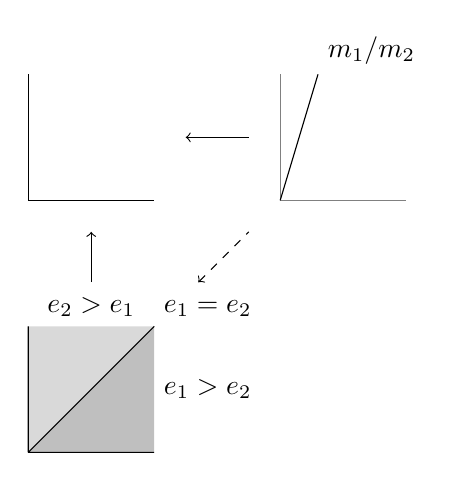
\begin{tikzpicture}[scale=0.8]
 \draw (0,0) -- (0,2)  (0,0)--(2,0);
 \draw[->] (1,-1.3) -- (1,-.5);
 \fill[gray!30] (0,-4) -- (0,-2) -- (2,-2) -- (0,-4);
 \fill[gray!50] (0,-4) -- (2,-4) -- (2,-2) -- (0,-4);
 \draw (0,-4) -- (0,-2) (0,-4) -- (2,-4) (0,-4) -- (2,-2) node[above right]{$e_1=e_2$};
 \draw (1,-2) node[above]{$e_2>e_1$} (2,-3) node[right]{$e_1>e_2$};
 \draw[<-] (2.5,1)--(3.5,1);
 \draw[gray!=30] (4,0) -- (4,2)  (4,0)--(6,0);
 \draw (4,0) -- (4.6,2) node[above right]{$m_1/m_2$};
 \draw[<-,dashed] (2.7,-1.3)--(3.5,-.5);
\end{tikzpicture}
\end{center}
So, for example, the factorisation exists for the subcone $e_2>e_1$ only when $m_1>m_2$, which is compatible with the fact that $\mathbb N^2=Q_{\rm{min}}^{\rm{prestable}}\to Q_{\rm{min}}^{\rm{log.map}}=\mathbb N$ is given by
$e_1\mapsto m_2, e_2\mapsto m_1$.
\end{example}

In fact we plan to work around the problem by directly looking at the desingularisation of the main component of Kim's moduli space of logarithmic maps to expanded targets.

\subsection{Logarithmic maps with expansions, alignments, factorisations} I will recall the basic definitions from \cite{KimLog,ChenDeg}; see also \cite{OlsCurves,AbramovichMarcusWiseComparison}. Essentially Kim's moduli space parametrises log morphisms to an expansion, where the minimal log structure on the base is locally free, twisted (in the sense that the irreducible elements are allowed to be roots of the smoothing parameters of the nodes in both the source and target), and identifies all the smoothing paramaters of the distinguished nodes of $C$ that map to the same component of the singular locus of $X^{\rm{exp}}=W$ (corank condition). Kim's moduli space should be thought of as the saturation of J. Li's moduli space. In the following $\pM_S^{C/S}$ denotes the log structure on the base $S$ pulled back from the canonical one on the moduli space of (pre)stable curves (i.e. the minimal log structure on the base of a family of log smooth curves), and similarly $\pM_S^{W/S}$.

\begin{definition}
 An \emph{extended log twisted expansion} of $(X,Y)$ is a quadruple $(\pi\colon W\to S, \pi_X\colon W\to X, D\subseteq W, \pM_S^{W/S}\to\pM_S)$ such that:
 \begin{enumerate}
  \item $\pi$ makes $W$ into a flat, proper algebraic space over $S$, with fibers at worst nodal in codimension 1, admitting a lifting to a special log morphism $\pi\colon (W,\pM_W^{W/S})\to(S,\pM_S^{W/S})$, such that:
  \begin{enumerate}
   \item $\pM_W^{W/S}$ and $\pM_S^{W/S}$ are locally free log structures;
   \item for every geometric point $\bar{w}\to W$, either $\bar{w}$ is in the smooth locus of $\pi_S$ and $\pi^\flat\colon \pi^*\overline{\pM}_{S,\bar{w}}^{W/S}\to \overline{\pM}_{W,\bar{w}}^{W/S}$ is an isomorphism, or $\bar{w}$ is in the nodal locus and the following diagram is cocartesian:
   \bcd
   \N\ar[r,"{(1,1)}"]\ar[d,"h"]\ar[dr,phantom,"\lrcorner"] & \N^2\ar[d] \\
   \pi^*\overline{\pM}_{S,\bar{w}}^{W/S}\ar[r] & \overline{\pM}_{W,\bar{w}}^{W/S}
   \ecd
   with $h(1)$ irreducible;
   \item for every geometric point $\bar{s}\to S$ there is a bijection between the irreducible elements of $\overline{\pM}_{S,\bar{s}}^{W/S}$ and the irreducible components of $W_{\bar{s}}^{\text{sing}}$.
  \end{enumerate}
  \item $D\subseteq W$ is a Cartier divisor, smooth over $S$, and such that $\pi_X(D)=Y$;
 \item $\pM_S$ is twisted by integers $(r_1,\ldots,r_l)$ and expanded with respect to $\pM_S^{W/S}$, namely \'{e}tale locally at every point $s\in S$ the morphism of log structures $\pM_S^{W/S}\to\pM_S$ admits a chart:
 \bcd
 \N^l\ar[d]\ar[r,"{(r_1,\cdots,r_l)}"] &\N^l\ar[r,"{(id,0)}"]&\N^l\oplus\N^k\ar[d] \\
 \pM_S^{W/S}\ar[rr] & & \pM_S
 \ecd
  
 \end{enumerate}
\end{definition}
 The log structure on $W$ is then given by
 \[ \pM_W=\pi^*\pM_S\oplus_{\pi^*\pM_S^{W/S}}\pM_W^{W/S}\oplus_{\OO^*_W}\pM^D\]
 where $\pM_D$ is the divisorial log structure associated to $D$. 
Notice that with this definition $(W,\pM_W)\to(S,\pM_S)$ is log smooth.

Similarly a \emph{log twisted curve} is $((C,p_1,\ldots,p_n)\to S, \pM_S^{C/S}\to\pM_S)$ with
\[\pM_C=\pi^*\pM_S\oplus_{\pi^*\pM_S^{C/S}}\pM_C^{C/S}\oplus_{\OO^*_C}\bigoplus_{i=1}^n\pM^{p_i}\]
A log twisted curve is \emph{minimal} if the log structure $\pM_S$ is locally free, and for every geometric point $\bar{s}\to S$ and irreducible element $b\in\overline{\pM}_S$, we can find an irreducible $a\in\overline{\pM}^{C/S}_S$ and a positive integer $l$ such that $a\mapsto lb$ (by definition this means that the morphism of log structures $\pM_S^{C/S}\to\pM_S$ is \emph{simple}).

Finally, fix an $n$-tuple of non-negative contact orders $(c_1,\ldots,c_n)$.
\begin{definition}
 A \emph{relative log prestable map} with tangency condition $\mathbf{c}$ is given by a diagram of log morphisms:
 \bcd
 ((C,\mathbf p),\pM_C)\ar[rr,"f"]\ar[dr] & & ((W,D),\pM_W)\ar[rr,"\pi_X"]\ar[dl] & & (X,Y)\times S \\
  & (S,\pM_S) & & &
 \ecd
 \begin{enumerate}
  \item $(C,\mathbf p),\pM_C)\to (S,\pM_S)$ is a minimal log twisted curve;
  \item $((W,\pM_W)\to (S,\pM_S),(W,D)\to(X,Y))$ is an extended twisted log expansion of $(X,Y)$;
  \item (\emph{corank condition}) for every geometric point $\bar{s}\in S$, the rank of \[\operatorname{Coker}(\pM^{W/S}_{S,\bar{s}}\to \pM_{S,\bar{s}})\] is equal to the number of non-distinguished nodes of $C_{\bar{s}}$; recall that a node of $C_{\bar{s}}$ is \emph{distinguished} if it is mapped under $f$ to the singular locus of $W_{\bar{s}}$.
  \item (\emph{log admissibility}) the morphism of log structures $f^\flat\colon f^*\pM_W\to\pM_C$ is simple at every distinguished node;
  \item (\emph{tangency condition}) the underlying map $\underline{f}\colon C\to (W,D)$ is non-degenerate, namely no component of $C$ is mapped entirely into $D$, and locally around every marking $p_i$ we can find a chart
  \bcd
  \N\ar[r,"\cdot c_i"]\ar[d] & \N\ar[d] \\
  f^*\pM^D\ar[r] & \pM^{p_i}
  \ecd
  for the restriction of $f^\flat$ to the $f^*\pM^D$ factor.
  \end{enumerate}
\end{definition}
\begin{definition}
 A relative log prestable map as above is \emph{stable} if for every geometric point $\bar{s}\in S$ the group of automorphisms $(\sigma,\tau)$ is finite, where:
 \begin{enumerate}
  \item $\sigma$ is an automorphism of $((C,\pM_C)\to (S,\pM_S))_{\bar{s}}$ preserving the markings $\mathbf p$;
  \item $\tau$ is an automorphism of $((W,\pM_W)\to (S,\pM_S))_{\bar{s}}$ preserving $D$ and $\pi_X\colon W_{\bar{s}}\to X$;
  \item $\tau\circ f_{\bar{s}}=f_{\bar{s}}\circ \sigma$.
 \end{enumerate}
\end{definition}
\begin{rmk}
 The corank and simplicity condition imply the following: the rank of the locally free log structure $\pM_S$ at $\bar{s}$ amounts to the number of irreducible components of $W_{\bar{s}}^{\text{sing}}$ plus the number of non-distinguished nodes of $C_{\bar{s}}$; all the smoothing parameters of the distinguished nodes mapping to the same component of $W_{\bar{s}}^{\text{sing}}$ have been identified \emph{up to twisting}. Indeed, at a distinguished node $q$ of $C$, letting $R$ be the local ring of $S$ at $\pi(q)$, we can find \'{e}tale local charts
 \bcd
 \N^2\oplus_{\N} \pM_{S}\ar[r,"{(id,\cdot m_q)}" below]\ar[d] & \N^2\oplus_{\N} \pM_{S}\ar[d] \\
 f^*\pM_W \ar[r,"f^\flat" below]\ar[d] & \pM_C\ar[d] \\
 R[z_1,\ldots,z_{\dim(X)-1},x,y]/(xy-t)\ar[r,"\left(\substack{x\mapsto a^{m_q}\\ y\mapsto b^{m_q}\\ t\mapsto s^{m_q}}\right)" below=.2cm] & R[a,b]/(ab-s)
 \ecd
 where the twist at $f(q)$ is given by $l$, the one at $q$ is given by $r_q$, and the equality $l=r_qm_q$ has to hold.
\end{rmk}
The following is a variation on \cite[\S 3.3]{RSPW2}. I will focus on the case of $(\PP^N|H)$.
\begin{definition}
 Let $(C,\mathbf p)\to (W,D)$ be a radially aligned Kim's log map to $(\PP^N|H)$, and let $\varphi\colon \plC\to\mathbb R_{\geq 0}$ be its tropicalisation, with circuit $\plC_0$. If $\varphi$ does not contract the circuit, set the contraction radius $\delta_f=0$. Otherwise let $\delta_f$ be the minimal distance from the circuit to a vertex supporting a flag that is not contracted by $\varphi$.
\end{definition}
To every Kim's log map we can associate an ordinary (not expanded) log map by collapsing the target and stabilising the curve \cite[Proposition 6.1]{GrossSiebertLog}. Furthermore, by choosing generic hyperplanes that meet the image of the curve transversally at smooth points of the latter, and by pulling back the resulting log structures on $\PP^N$, we may lift any log map to $(\PP^N|H)$ to one to $(\PP^N|\Delta)$, where $\Delta$ denotes the toric boundary of $\PP^N$. Notice that, when looking at the tropicalisation, any generic choice of hyperplanes will add flags only to vertices that already have a non-contracted flag, hence the resulting $\delta_f^{\Delta}$ is the same as $\delta_f$, and does not depend on this choice.

It is discussed in \cite[Proposition 2.4.2.1]{RSPW2} how log morphisms from an fs log scheme $C\to Z$, where $Z$ is a toric variety with the log structure associated to its boundary, are equivalent to the data of $M\xrightarrow{\alpha} H^0(C,\pM_C^{\rm{gp}})$, such that for every $x\in C$ we can find a cone $\sigma$ in the fan of $Z$ and a factorisation:
\bcd
M\ar[r] & H^0(C,\pM_C^{\rm{gp}})\ar[r] & \overline{\pM}_{C,x}^{\rm{gp}} \\
S_\sigma\cap M\ar[u,hook]\ar[rr,dashed] & & \overline{\pM}_{C,x}\ar[u,hook]
\ecd
where $M$ is the character lattice of the torus $T\subseteq Z$, and $S_\sigma$ is the dual cone of $\sigma$. This is useful because it allows them to impose factorisation of $C\to Z\dashrightarrow \PP^1$ to the Smyth's singularity determined by $\delta_f^\Delta$ without having to modify $Z$ (and $C$, and $S$), see \cite[Definition 3.3.3]{RSPW2}.
\begin{dfn}
 A log map $f\colon C\to Z$ from an aligned curve to a toric variety satisfies the factorisation property for a subtorus $H\subseteq T$ if the associated composition \[M_{T/H}\to M\xrightarrow{\alpha} H^0(C,{\pM}_C^{\rm{gp}})\to H^0(\widetilde{C},\pM_{\widetilde{C}}^{\rm{gp}})\] descends to $M_{T/H}\to H^0(\overline{C},\pM_{\overline{C}}^{\rm{gp}})$, where the modification and contraction $C\leftarrow \widetilde{C}\to \overline{C}$ are determined by the contraction radius $\delta_{\alpha}$, that is the largest distance of a vertex to the circuit such that the line bundle associated to $\bar\alpha$ is trivial on the interior of the circle of radius $\delta_\alpha$.
 
 A map $f\colon C\to Z$ is called well-spaced if it satisfies factorisation for every subtorus $H\subseteq T$.
\end{dfn}

\begin{dfn}
 Let $\alpha\in\N^n$ be a maximal tangency condition. The space $\VZK{\alpha}{\PP^N|H}{d}$ parametrises Kim's log maps from an aligned curve to an expansion such that the associated log map to $(\PP^N|\Delta)$ (for any generic choice of hyperplanes $H_1,\ldots,H_N$) satisfies well-spacedness.
\end{dfn}

I claim that this construction provides a desingularisation of the main component of Kim's space in genus one: indeed it includes the locus of maps from a smooth elliptic curve whose image is not contained in $H$, and on the other hand its smoothness can be argued as follows. The morphism $\VZK{\alpha}{\PP^N|H}{d}\to \VZa{\alpha}{\PP^N|H}{d}$ is toroidal (this can be argued from \cite[Lemma A and \S 4.3]{AbramovichMarcusWiseComparison} and the analogous statement for the universal target). On the other hand, locally we may find $U_{\VZK{\alpha}{\PP^N|\Delta}{d}}\to U_{\VZK{\alpha}{\PP^N|H}{d}}$ which is \'etale by the infinitesimal criterion (lifting is tantamount to deforming the extra hyperplanes $H_1,\ldots,H_n$). We are then reduced to \cite[Theorem 3.5.1]{RSPW2}.

\subsection{Description of the boundary} As in Gathmann's work, there is a line bundle with section that forces the $k$-th marked point to have tangency of order $\alpha_k+1$ to $H$, which in the maximal tangency situation and in the expanded setup (as is the case for us) really forces the target to break, and the $k$-th marking $x_k$ to lie on a non-trivial component mapped to the highest level of the accordion. The line bundle and section $(\mathcal L_{\alpha,k},s_{\alpha,k})$ are the pullback of $(x_k^*\Omega_{C}^{\otimes \alpha_k+1}\otimes\ev_1^*\OO_\PP^N(1),\ev_k^*(d^{\alpha_k+1}s))$ from the collapsed and stabilised map. The description of the boundary in the case of $(\PP^N|H)$ boils down to a dimension computation, and is already present in the work of Vakil \cite{Vre}. There are three relevant combinatorial types, corresponding to bipartite graphs:
\begin{enumerate}[label=(\alph*)]
 \item $\Yagraph$ \begin{multline*}\mathcal Y^a=\left(\VZ{\alpha^{(1)}\cup\{m^{(1)}\}}{\PP^N|H}{d_1}\times\prod_{i=2}^r\M{0}{\alpha^{(i)}\cup\{m^{(i)}\}}{\PP^N|H}{d_i}\right)\times_{H^r} \\ \M{0}{(-m^{(1)},\ldots,-m^{(r)})\cup\alpha^{(0)}}{\PP_H(\OO\oplus\OO(1)}{d_0}^\thicksim\end{multline*}
 \item $\Ybgraph$ \begin{multline*}\mathcal Y^b=\left(\M{0}{\alpha^{(1)}\cup\{m^{(1)},m^{(2)}\}}{\PP^N|H}{d_1}\times\prod_{i=3}^r\M{0}{\alpha^{(i)}\cup\{m^{(i)}\}}{\PP^N|H}{d_i}\right)\times_{H^r}\\ \M{0}{(-m^{(1)},-m^{(2)}\ldots,-m^{(r)})\cup\alpha^{(0)}}{\PP_H(\OO\oplus\OO(1)}{d_0}^\thicksim\end{multline*}
 \item $\Ycgraph$\begin{multline*}\mathcal Y^c= \prod_{i=1}^r\M{0}{\alpha^{(i)}\cup\{m^{(i)}\}}{\PP^N|H}{d_i}\times_{H^r}\VZdrc{(-m^{(1)},\ldots,-m^{(r)})\cup\alpha^{(0)}}{\PP_H(\OO\oplus\OO(1)}{d_0}^\thicksim\end{multline*}
\end{enumerate}
A few remarks on the notation are in order: a white circle in the graphs always stands for a genus one component; the tilde denotes moduli spaces of rubber maps, which were introduced in \cite{GraberVakil} (material on how they compare to the ordinary moduli space of maps to the underlying $H$ can be found in \cite[Chapter 5]{GathmannThesis}). DRC stands for ``double ramification cycle'', i.e. for the extra equation in $\Pic$ that needs to be satisfied:
\[f_{|E}^*\mathcal O_H(1)\cong\mathcal O_E\left(\sum_{x_j\in E}\alpha_jx_j-\sum_{i=1}^r m^{(i)}y_i\right).\]
In genus one this is a divisorial condition, and an explicit tautological formula was already known to R. Hain \cite{Hain} (later confirmed and generalised in \cite{JPRZ}); what we can do exploiting Gathmann's argument is computing (relating) a number of $\psi$-integrals against the DRC, more in the spirit of \cite{BSZ}. It is worth subdividing case (c) above into $\mathcal Y^c_+$ (for $d_0>0$) and $\mathcal Y^c_0$ (for $d_0=0$): notice that the generic element of the latter is already aligned (indeed the minimal monoid is $\N$, since all the nodes are distinguished and map to the same component of the singular locus of the target); on the other hand we need to impose the well-spacedness condition, which will hopefully be expressible as a tautological integral, based on the analysis of Lemma \ref{lem:fundamental}. The data above depend on a splitting $(A,B,M)$ of the markings, degree, and external multiplicities, such that $d_0+\sum m^{(i)}=\sum A^{(0)}$, and factorisation should impose $N-1$ independent conditions, unless all the $m^{(i)}\geq 2$, in which case there are only $N-2$ conditions (this would be the dimensionally relevant case). Finally, let me observe that all the insertions that we are interested in are pulled back from the moduli space of maps to the collapsed target, hence any locus with positive-dimensional fibers for the collapsing may be overlooked; this is the case when there is more than one non-trivial component mapping to higher level in the accordion, which is the reason why only the three graph types above appear. All the boundary divisors appear in the vanishing locus of $s_{\alpha,k}$ with positive multiplicity $\frac{m^{(1)}\cdots m^{(r)}}{r!}$ (the $r!$ is only there to make the gluing nodes unordered), as already predicated in \cite{Vre} and discussed in Remark \ref{rmk:expandedGathmann}.

The formula in the case of non-maximal tangency can be proven by adding $h=d-\sum\alpha$ auxiliary markingsof multiplicity $(1,\ldots,1)$, and then forgetting them (which is generically a $h!\colon 1$ cover), pretty much along the lines of \cite[Corollary 3.5]{Ga}. Importantly, the difference between $\psi_k$ on the space with auxiliary markings and $\fgt_{n+1,\ldots,n+h}^*\psi_k$ can be expressed in terms of boundary classes. It may be useful to notice that as soon as there is more than one non-trivial component at higher level, or the only such component has zero horizontal degree and contains more than one of the auxiliary markings, then the corresponding locus has positive-dimensional fibers for forgetting $x_{n+1},\ldots,x_{n+h}$ and collapsing. Also, forgetting a point on the genus one component at level one in case (c) may make the difference between having to impose the DRC condition or not. So after all the general formula takes the following shape:
\begin{multline*}(\alpha_k\psi_k+\ev_k*H)\cap[\VZ{\alpha}{\PP^N|H}{d}]=[\VZ{\alpha+e_k}{\PP^N|H}{d}]+\\ \sum_{(I)}[\mathcal Y_a]+\sum_{(I)}[\mathcal Y_b]+\sum_{(I)}[\mathcal Y_c]+\sum_{(II)}[\mathcal Y_c^{\rm{no DRC}}]\end{multline*}
where $(I)$ and $(II)$ range over all the splittings $(A,B,M)$ such that $\alpha_k\in A^{(0)}$ and
\begin{enumerate}[label=(\Roman*)]
 \item $d_0+\sum m^{(i)}=\sum A^{(0)}$,
 \item $d_0+\sum m^{(i)}=\sum A^{(0)}+1$.
\end{enumerate}

\subsection{Examples}